\chapter{相关工作}\label{chap:relate}

本章的主要内容分为三个部分,第一部分主要介绍微表情研究中使用的数据集以及微表情和常见的宏表情之间的差异,第二部分介绍近几年微表情研究中所使用的特征提取的几种方法,第三部分介绍本文将在第四章中使用的相关深度网络的基础知识。

\section{宏表情和微表情}

普通的人脸表情可以是自然产生的,也可以是根据需要人为的摆拍出来。摆拍的人脸表情是有意表现出某种情绪,而自然产生的人脸表情是在表达自己的真实情感。所以在人脸宏表情(普通人脸表情)的研究中,既有自然产生的表情数据,也有摆拍的表情数据,微表情研究也存在类似的问题。在微表情研究领域用“自发”这个词来强调微表情的产生(或被诱导)是自然的,因为参与者的内心存在实际的情感。

所以根据表情的产生方式将微表情分为“自发”产生的真实微表情和“摆拍”的微表情。目前摆拍的数据集主要有USF-HD数据集和Polikovsky数据集,自然状态下诱发产生的自发数据集,主要包括SMIC、SMIC2、CASME、CASME II和SAMM等数据集,本节将简单介绍几种数据集的产生方式和优缺点,同时列举典型的宏表情数据集做对比,明确微表情的概念。。

\subsection{宏表情数据集}

随着图像识别和表情研究的深入,宏表情数据集的建立越来越完备。目前常用的人脸宏表情数据集有日本女性表情库(The Japanese female facial expression,JAFFE)\citep{Lyons2002Coding}、Yale表情数据集\citep{Belhumeur2002Eigenfaces}和CK+人脸表情数据集\citep{Lucey2010The}等。本文提出的算法中没有用到宏表情,此处以最常用的CK+数据集举例只为说明宏表情和微表情之间的差异。

CK+数据集是在Cohn-Kanade Dataset的基础上扩展来的,发布于2010年。2000年,Cohn-Kanade(CK)数据集发布,目的是促进人脸面部表情的自动检测研究。从那时起,CK数据集成为算法开发和评估中使用最广泛的测试平台之一。在此期间,产生了三个明显的局限性:1)虽然AU编码经过了很好的验证,但是情感标签是错误的,因为标定的标签是被要求的,而不是实际产生的;2)对新算法的评估缺乏一个通用的性能指标;3)不包含常见数据集的标准协议。因此,CK数据集被用于AU和情感检测时缺少与基准算法的比较,并且使用原始数据集的随机子集使得对元数据的分析变得困难。为了解决这些问题,发布了扩展版的Cohn-Kanade数据集CK+。CK+数据集中的表情分为三类,包括了摆拍和自发的表情以及其他类型的元数据(Metadata)。对于摆拍的表情,序列的数量比第一版的增加了22\%,参与者的数量增加了27\%。与初始版本一样,每个序列的目标表情都是完整的FACS编码,情感标签也经过了修改和验证。此外,元数据中还添加了经过验证的情感标签。数据集中还包含使用主动外观模型(Active Appearance Models,AAMs)和线性支持向量机分类器给出的基线结果,使用留一法交叉验证对摆拍的数据进行AU和情绪检测。

CK+数据集包括123个参与者,593个图像序列,每个图像序列的最后一张帧有AU标签,而在这593个图像序列中,有327个序列有情感标签。CK+数据集是人脸表情识别中比较流行的一个数据集,该数据集将情感分为8类,包括中性,厌恶,愤怒,蔑视,恐惧,高兴,悲伤,惊讶。图~\ref{fig1}给出了该数据集中的样本图片。综合来说,CK+是目前较为理想的表情数据集。

\begin{figure}[!htbp]
    \centering
    \begin{subfigure}[b]{0.22\textwidth}
      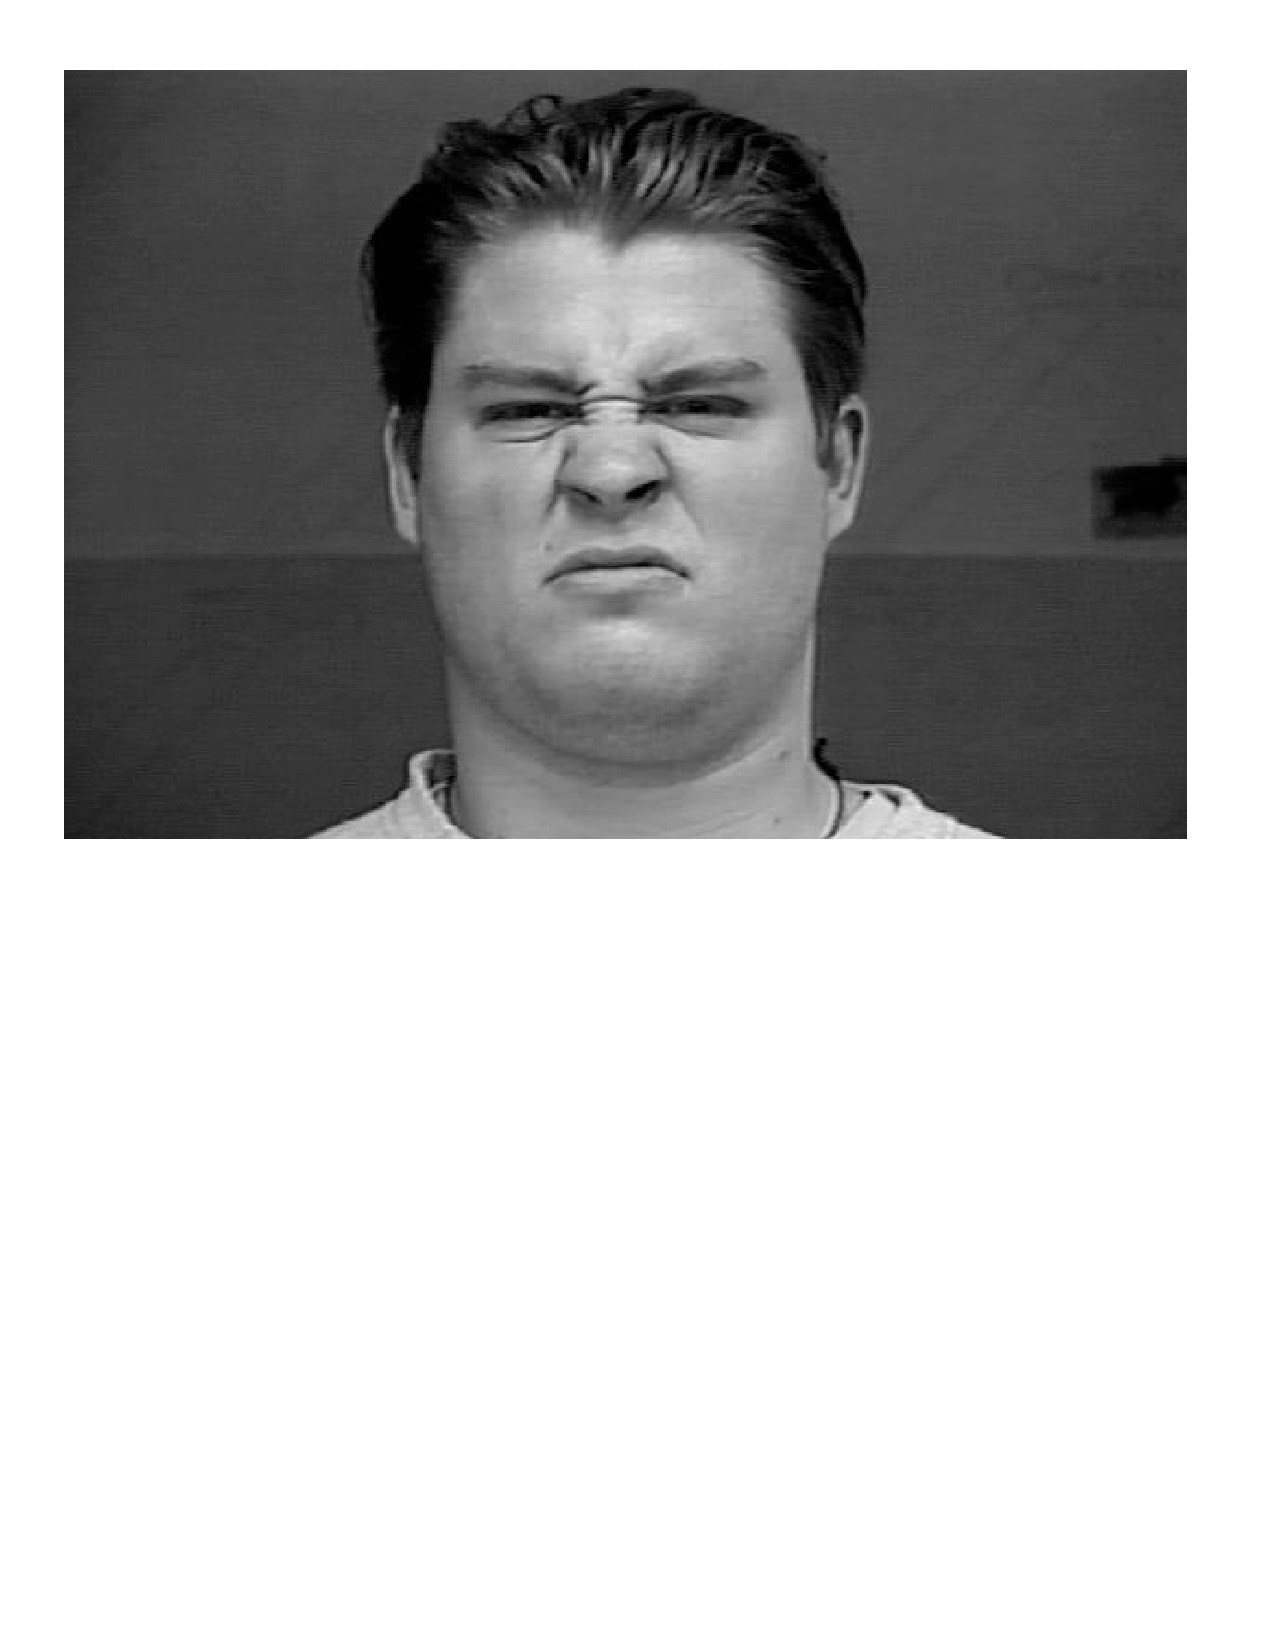
\includegraphics[width=\textwidth]{ME31}
      \caption{}
      \label{fig3.1}
    \end{subfigure}%
    ~%add desired spacing
    \begin{subfigure}[b]{0.22\textwidth}
      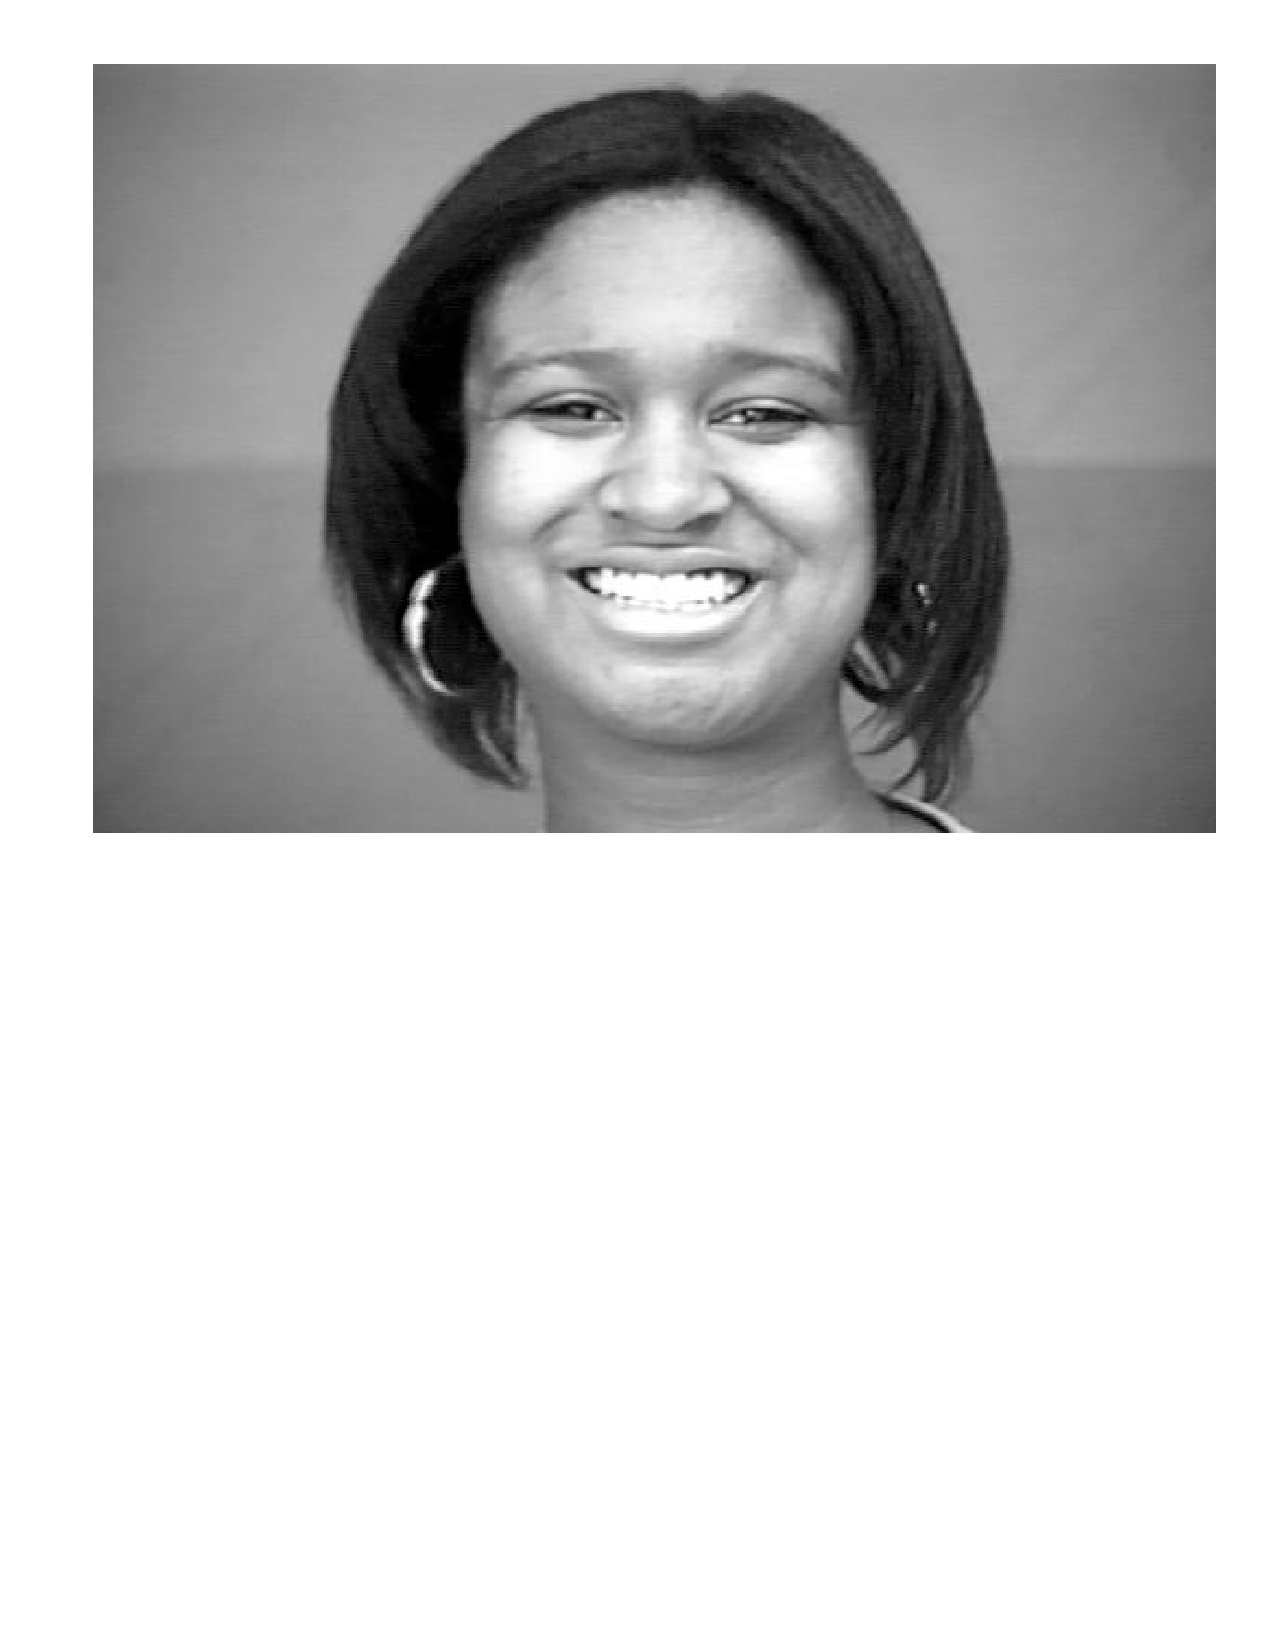
\includegraphics[width=\textwidth]{ME32}
      \caption{}
      \label{fig3.2}
    \end{subfigure}
    \begin{subfigure}[b]{0.22\textwidth}
      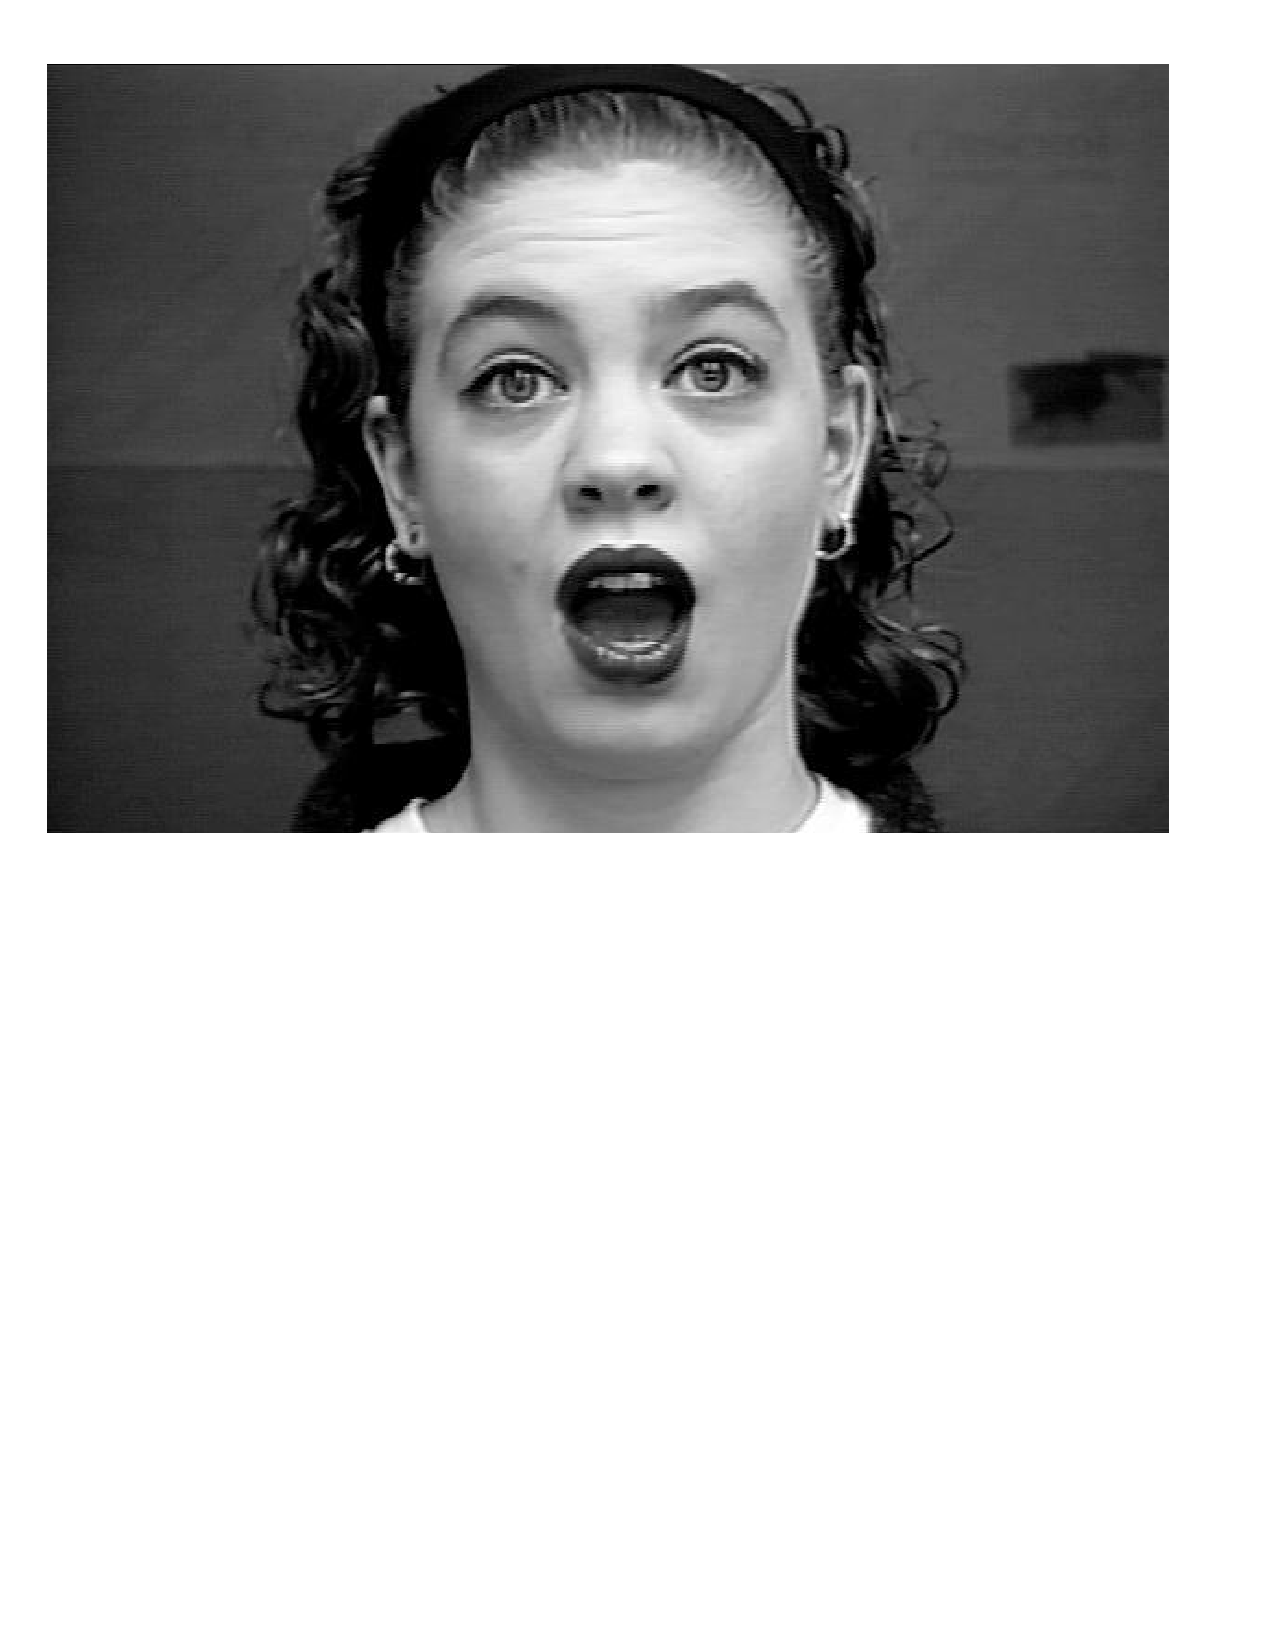
\includegraphics[width=\textwidth]{ME33}
      \caption{}
      \label{fig3.3}
    \end{subfigure}%
    ~%add desired spacing
    \begin{subfigure}[b]{0.22\textwidth}
      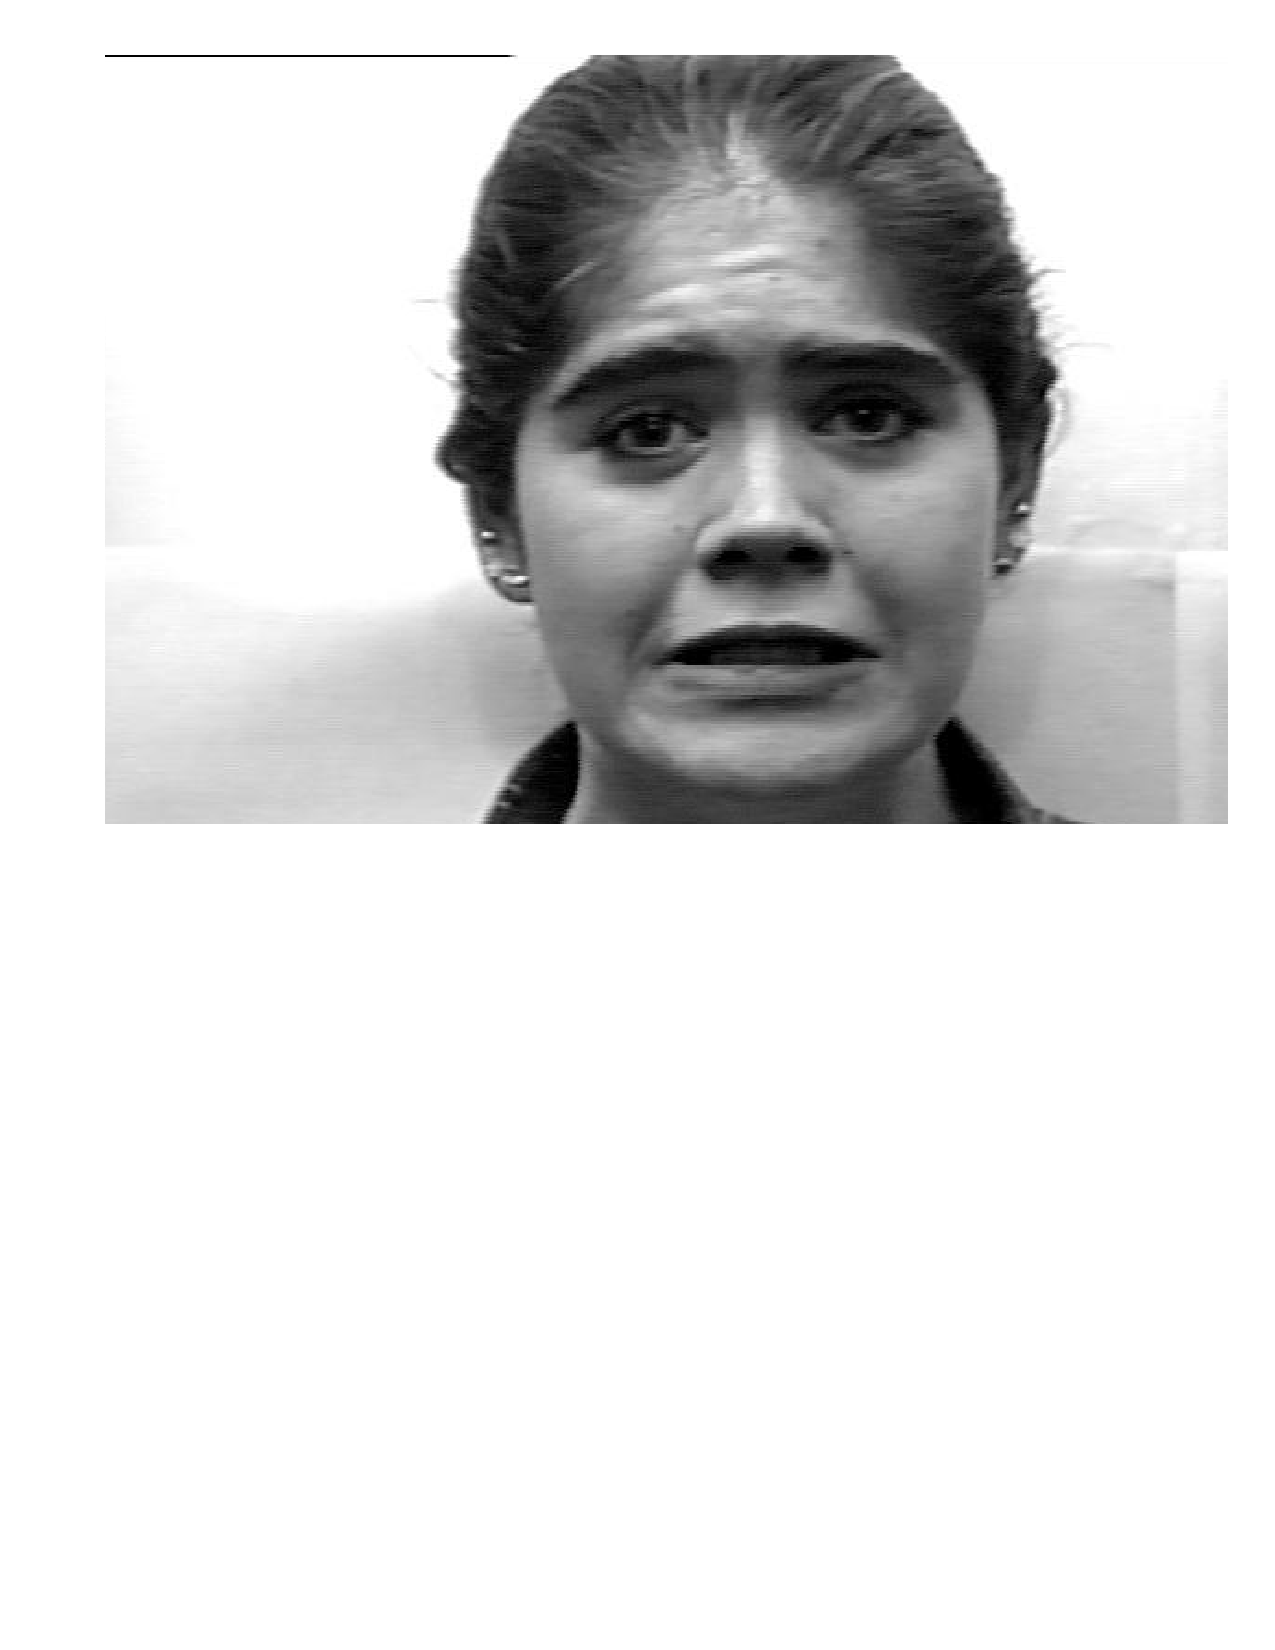
\includegraphics[width=\textwidth]{ME34}
      \caption{}
      \label{fig3.4}
    \end{subfigure}
    \begin{subfigure}[b]{0.22\textwidth}
      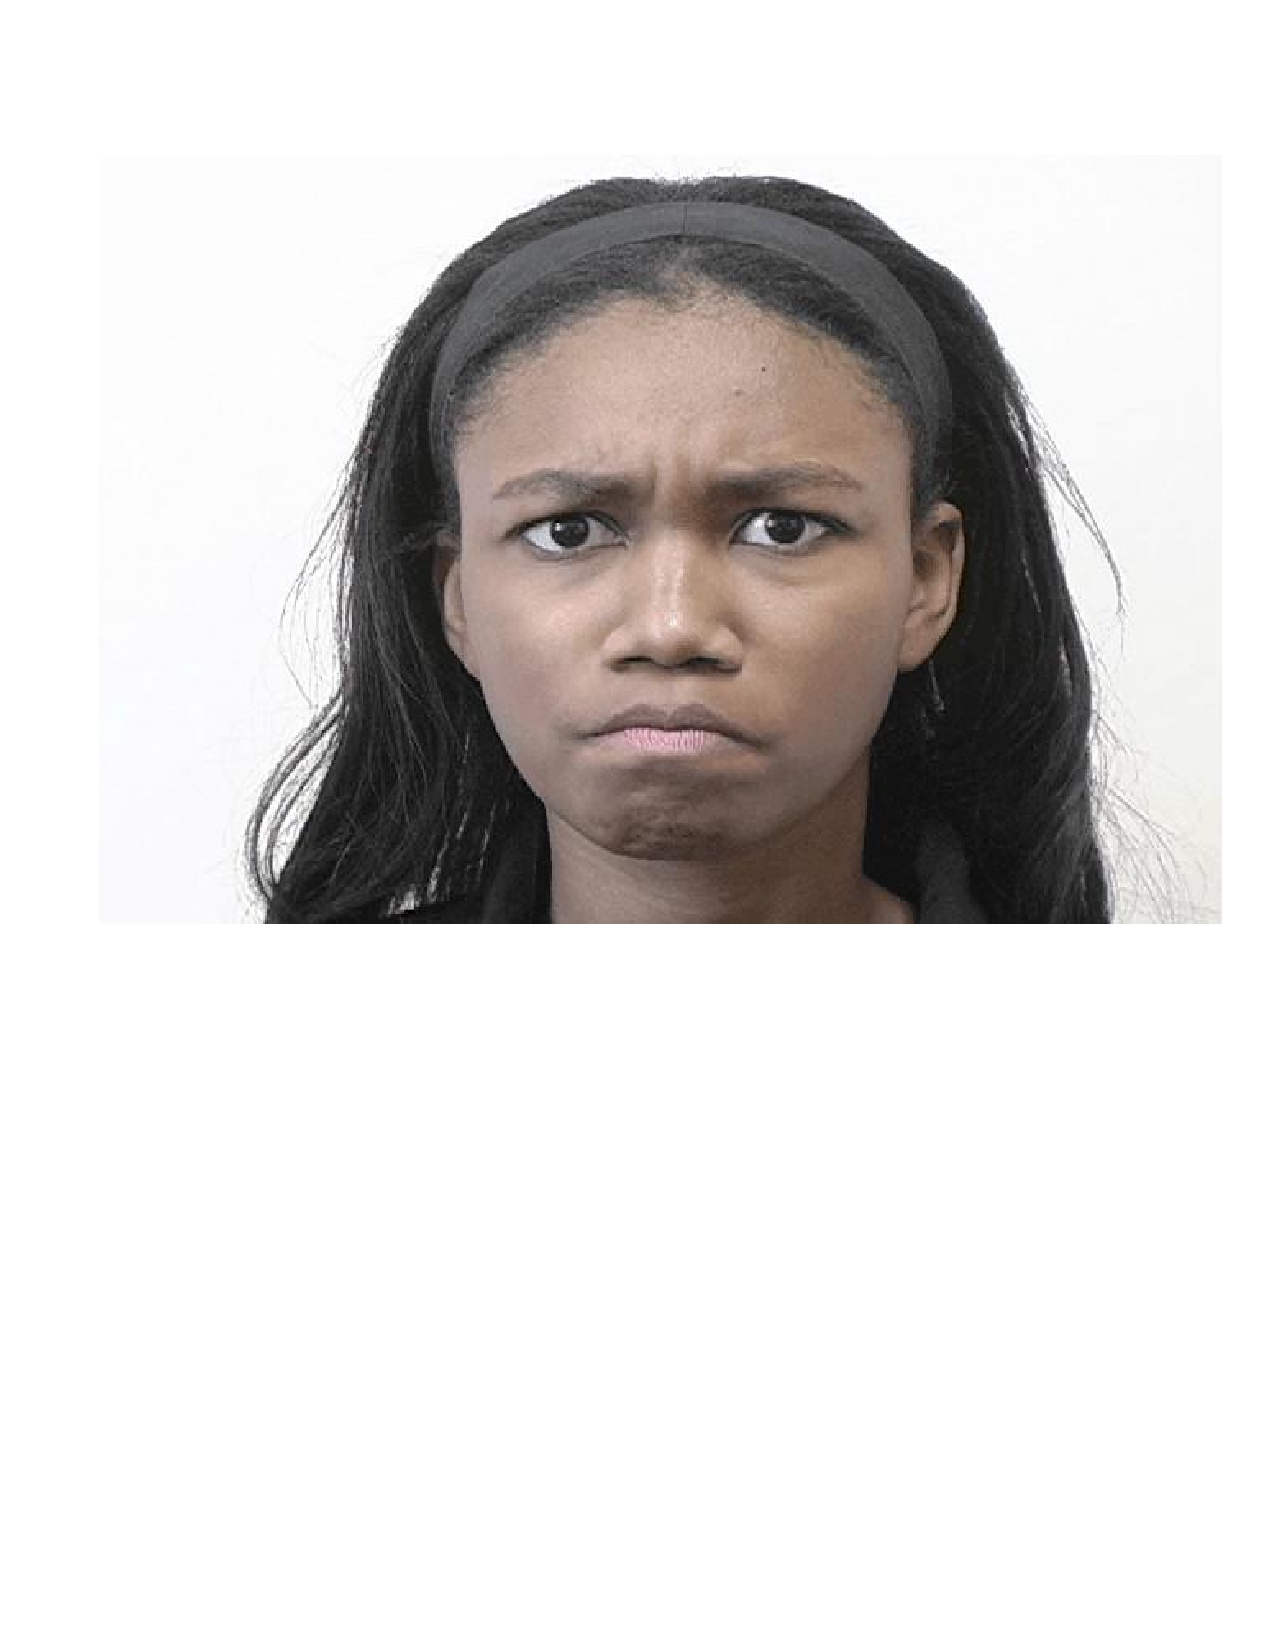
\includegraphics[width=\textwidth]{ME35}
      \caption{}
      \label{fig3.5}
    \end{subfigure}
    \begin{subfigure}[b]{0.22\textwidth}
      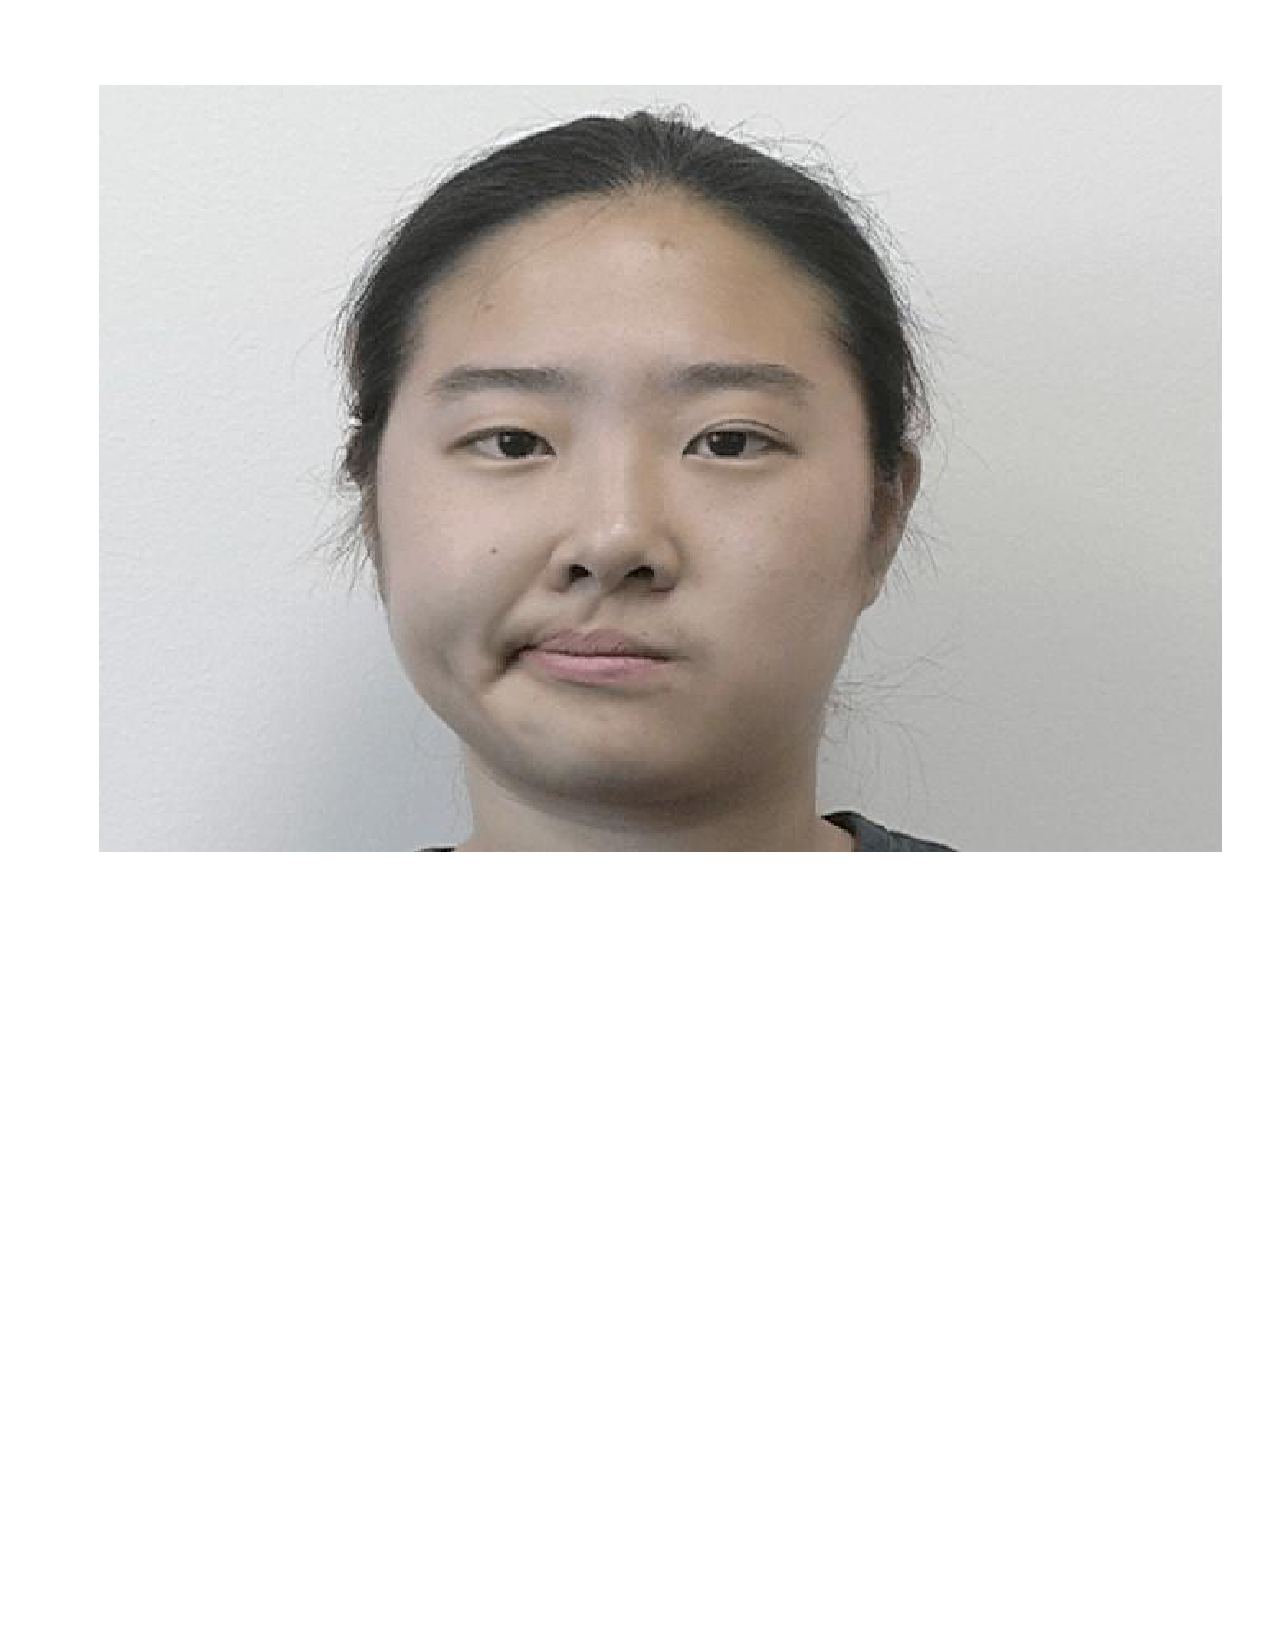
\includegraphics[width=\textwidth]{ME36}
      \caption{}
      \label{fig3.6}
    \end{subfigure}
    \begin{subfigure}[b]{0.22\textwidth}
      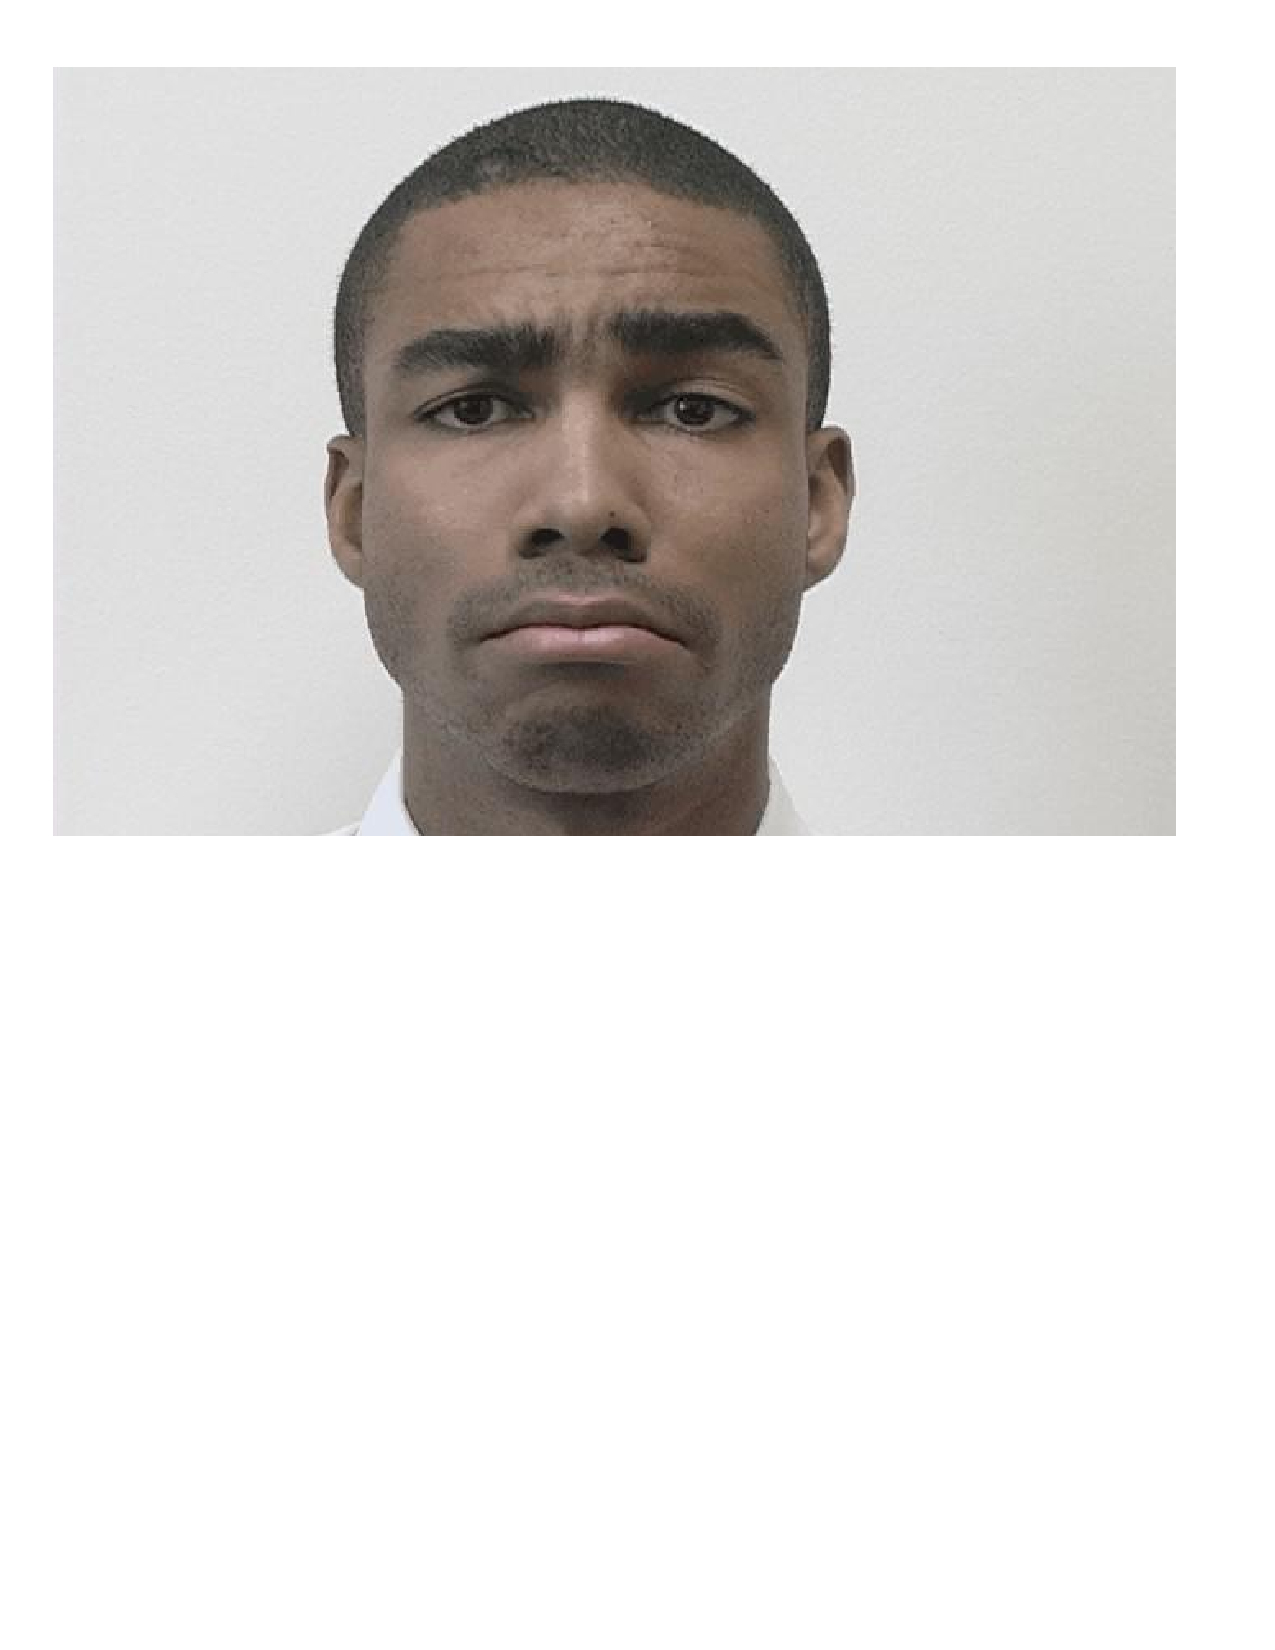
\includegraphics[width=\textwidth]{ME37}
      \caption{}
      \label{fig3.7}
    \end{subfigure}
    \begin{subfigure}[b]{0.22\textwidth}
      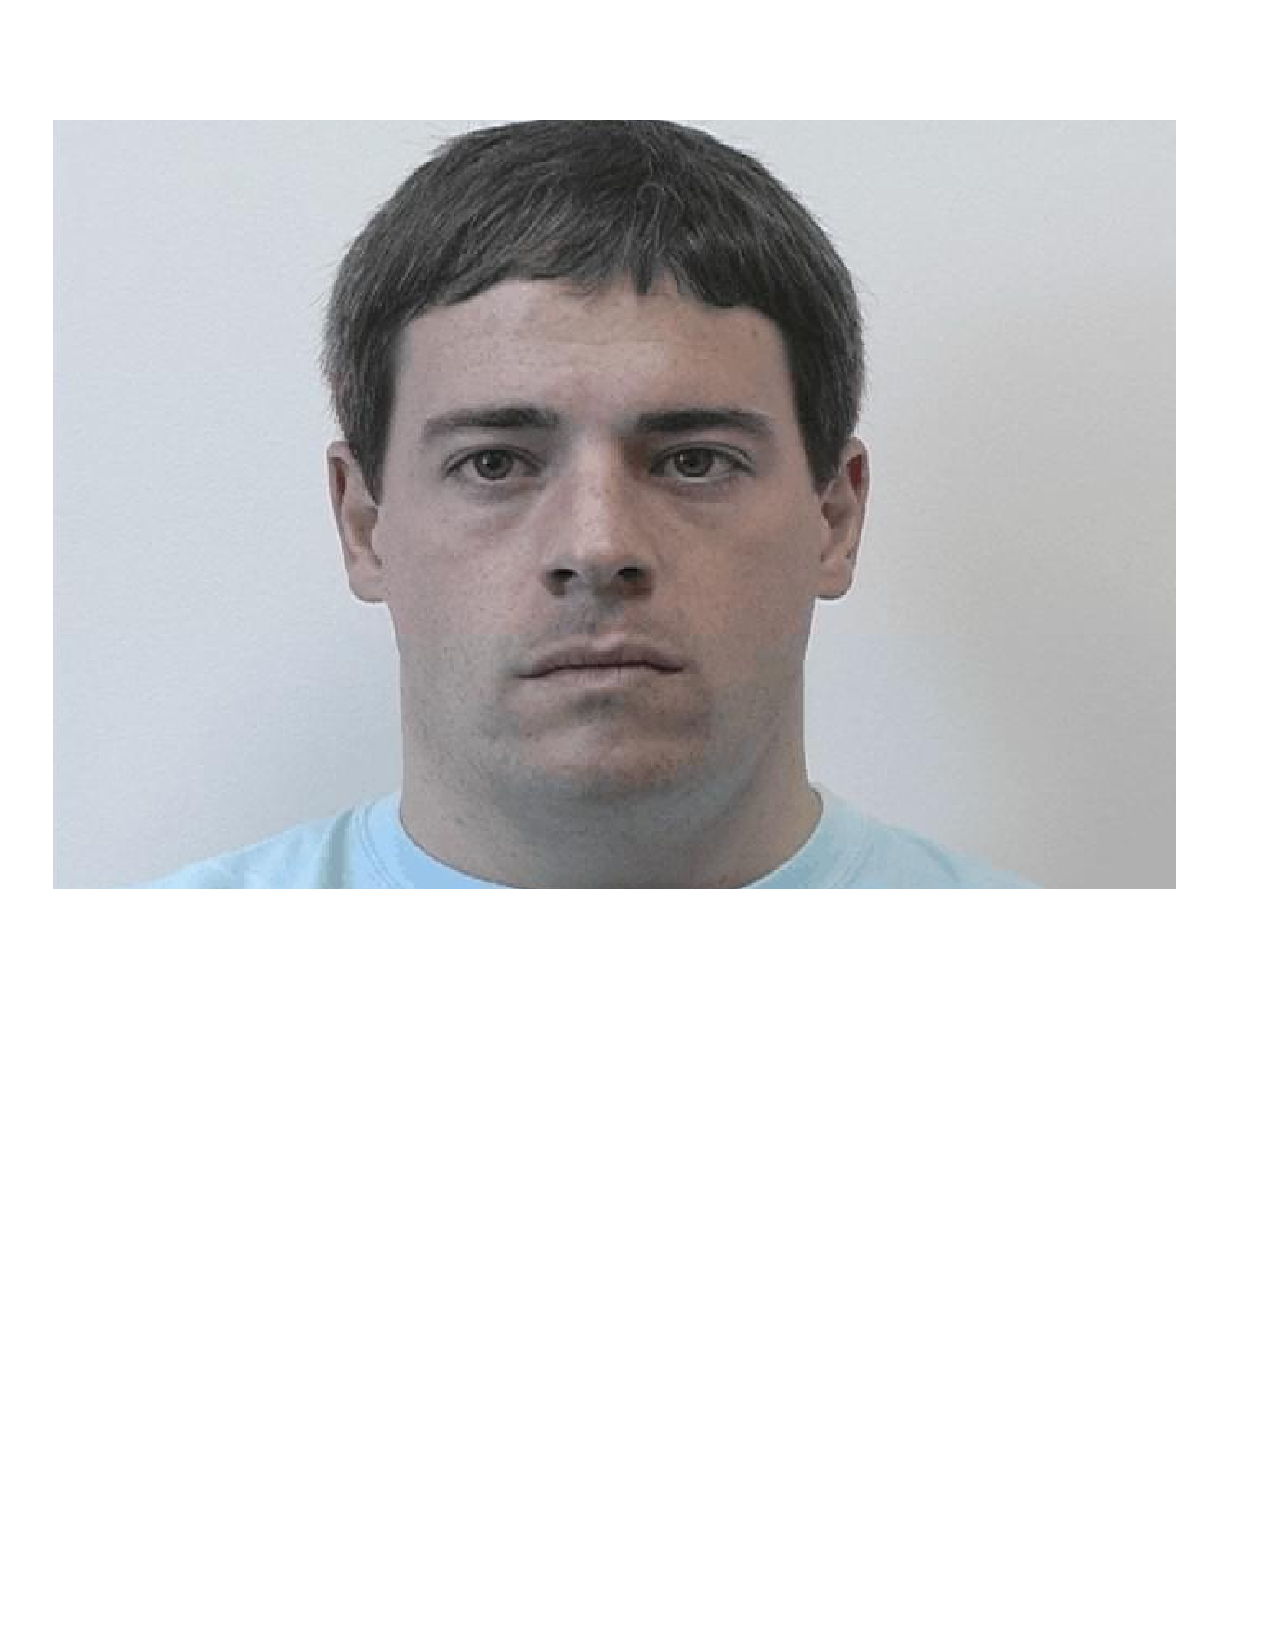
\includegraphics[width=\textwidth]{ME38}
      \caption{}
      \label{fig3.8}
    \end{subfigure}
    \caption{人脸宏表情样本示例(CK+数据集)
            (a)厌恶, (b)快乐, (c)惊讶, (d)恐惧, (e)愤怒, (f)轻蔑, (g)沮丧, (h)中性表情}
    \label{fig1}
\end{figure}

\subsection{早期微表情数据集}

由于微表情在镜头下很难产生,所以微表情数据的缺乏是微表情研究的第一障碍。虽然微表情已经被心理学家研究了很长一段时间,但网络上广泛传播的微表情样本仅仅只有片段,并没有发现任何心理学研究小组分享的大数据集。作者认为第一个原因是心理学研究更关注微表情本身的性质,比如什么时候出现或者看起来是什么样子,所以他们不需要像使用计算机研究那样需要大量的微表情数据。其次,在某些情况即使涉及到大量的微表情数据,但由于保密性限制,数据无法公开共享,例如患者的病历或司法讯问记录等。

以2009年为时间点,在此以前属于微表情的早期研究阶段,一些研究人员在他们的研究中使用了摆拍的微表情数据,这些数据避免了自发微表情数据获取时的困难,作为早期自动微表情识别研究的尝试,使用摆拍的数据是一次历史性的突破。例如Shreve等人收集了一个名为USF-HD的数据集,其中包含100个摆拍的微表情片段,视频长度平均在1分钟左右,最长2分钟,最短20秒。研究人员要求参与者模仿屏幕上显示的微表情样本作为数据的来源,同时在他们的文章中明确写到可以通过要求参与者尽可能快地模仿来收集一个摆拍的微表情数据集。Polikovsky等人也收集了一个摆拍的微表情数据集,要求受试者在低强度下表演七种基本情绪,并尽快回到中性表情,数据由一台每秒200帧的高速摄像机记录。表~\ref{tab3}列出了摆拍的微表情数据集的详细属性。

\begin{table}[!htbp]
\centering
\caption{摆拍微表情数据集}
\label{tab3}
\footnotesize% fontsize
\setlength{\tabcolsep}{4pt}% column separation
\renewcommand{\arraystretch}{1.2}%row space
\begin{tabular}{c|cc}
\hline
 & USF-HD & Polikovsky \\ \hline
微表情片段 & 100 & N/A \\
参与者 & N/A & 10 \\
分辨率 & $720\times1280$ & $480\times640$ \\
FPS & 29.7 & 200 \\
FACS & NO & YES \\
表情类 & N/A & 7 \\
人种 & N/A & 3 \\ \hline
\end{tabular}
\end{table}

值得注意的是摆拍的微表情数据不可以代替或与自发的微表情数据一起使用,因为这两种数据是不同性质的。例如在研究微表情的起始点时,由于两者是在不同的机制下产生的,所以摆拍的微表情在时空特性上与自发的微表情存在很大的差异,其次在研究视频的上下文时,由于模仿的表情与通过视频编辑生成的摆拍微表情片段通常在起止点很突兀,而且期间禁止其他无关的动作发生,这也与自发的微表情有很大的不同。另一方面,自然环境下自发的微表情可能伴随着复杂的场景,比如头部运动和眨眼等动作。基于这些事实,利用摆拍的微表情数据进行研究并不能真正解决实际中微表情分析的自动化问题,所以努力收集自发的微表情数据是后续工作的正确路径。需要说明的是在本文接下来的内容中,所有的工作都是关于自发微表情的,如果没有特别说明,“微表情”一词表示自发微表情。

\subsection{自发微表情数据集}

A. SMIC数据集介绍

2011年,论文\citepns{pfister2011recognising}首次提出了一种诱导和收集自发微表情的方法,将获得的数据集命名为“自发微表情语料库”,简称SMIC,它是第一个使用自然诱发状态的微表情数据集,对后续的数据集建立具有很好的指导性意义。第一版的SMIC数据集只包含了6位参与者的数据,论文\citepns{Li2013A}对其进行了扩充,包含了16名参与者的164个自发微表情片段,由三种相机记录的3个数据集组成:100fps的高速相机记录的HS数据集、25fps的普通彩色相机记录的VIS数据集和25fps的近红外摄像机记录的NIR数据集,且所有数据集具有相同的图像分辨率$640\times480$。增加VIS和NIR摄影机有三个考虑:(1)提升数据集的多样性;(2)研究高速相机在微表情分析方面是否优于普通速度相机;(3)研究时间插值方法是否可以应用于普通高速相机,以解决相机的短时插值问题。图~\ref{fig2}给出一个消极的微表情序列,通过该样例可以看出,一个微表情是由一组图片序列构成的,本样例的变化主要表现为嘴角的细微下沉。

\begin{figure}[!htbp]
    \centering
    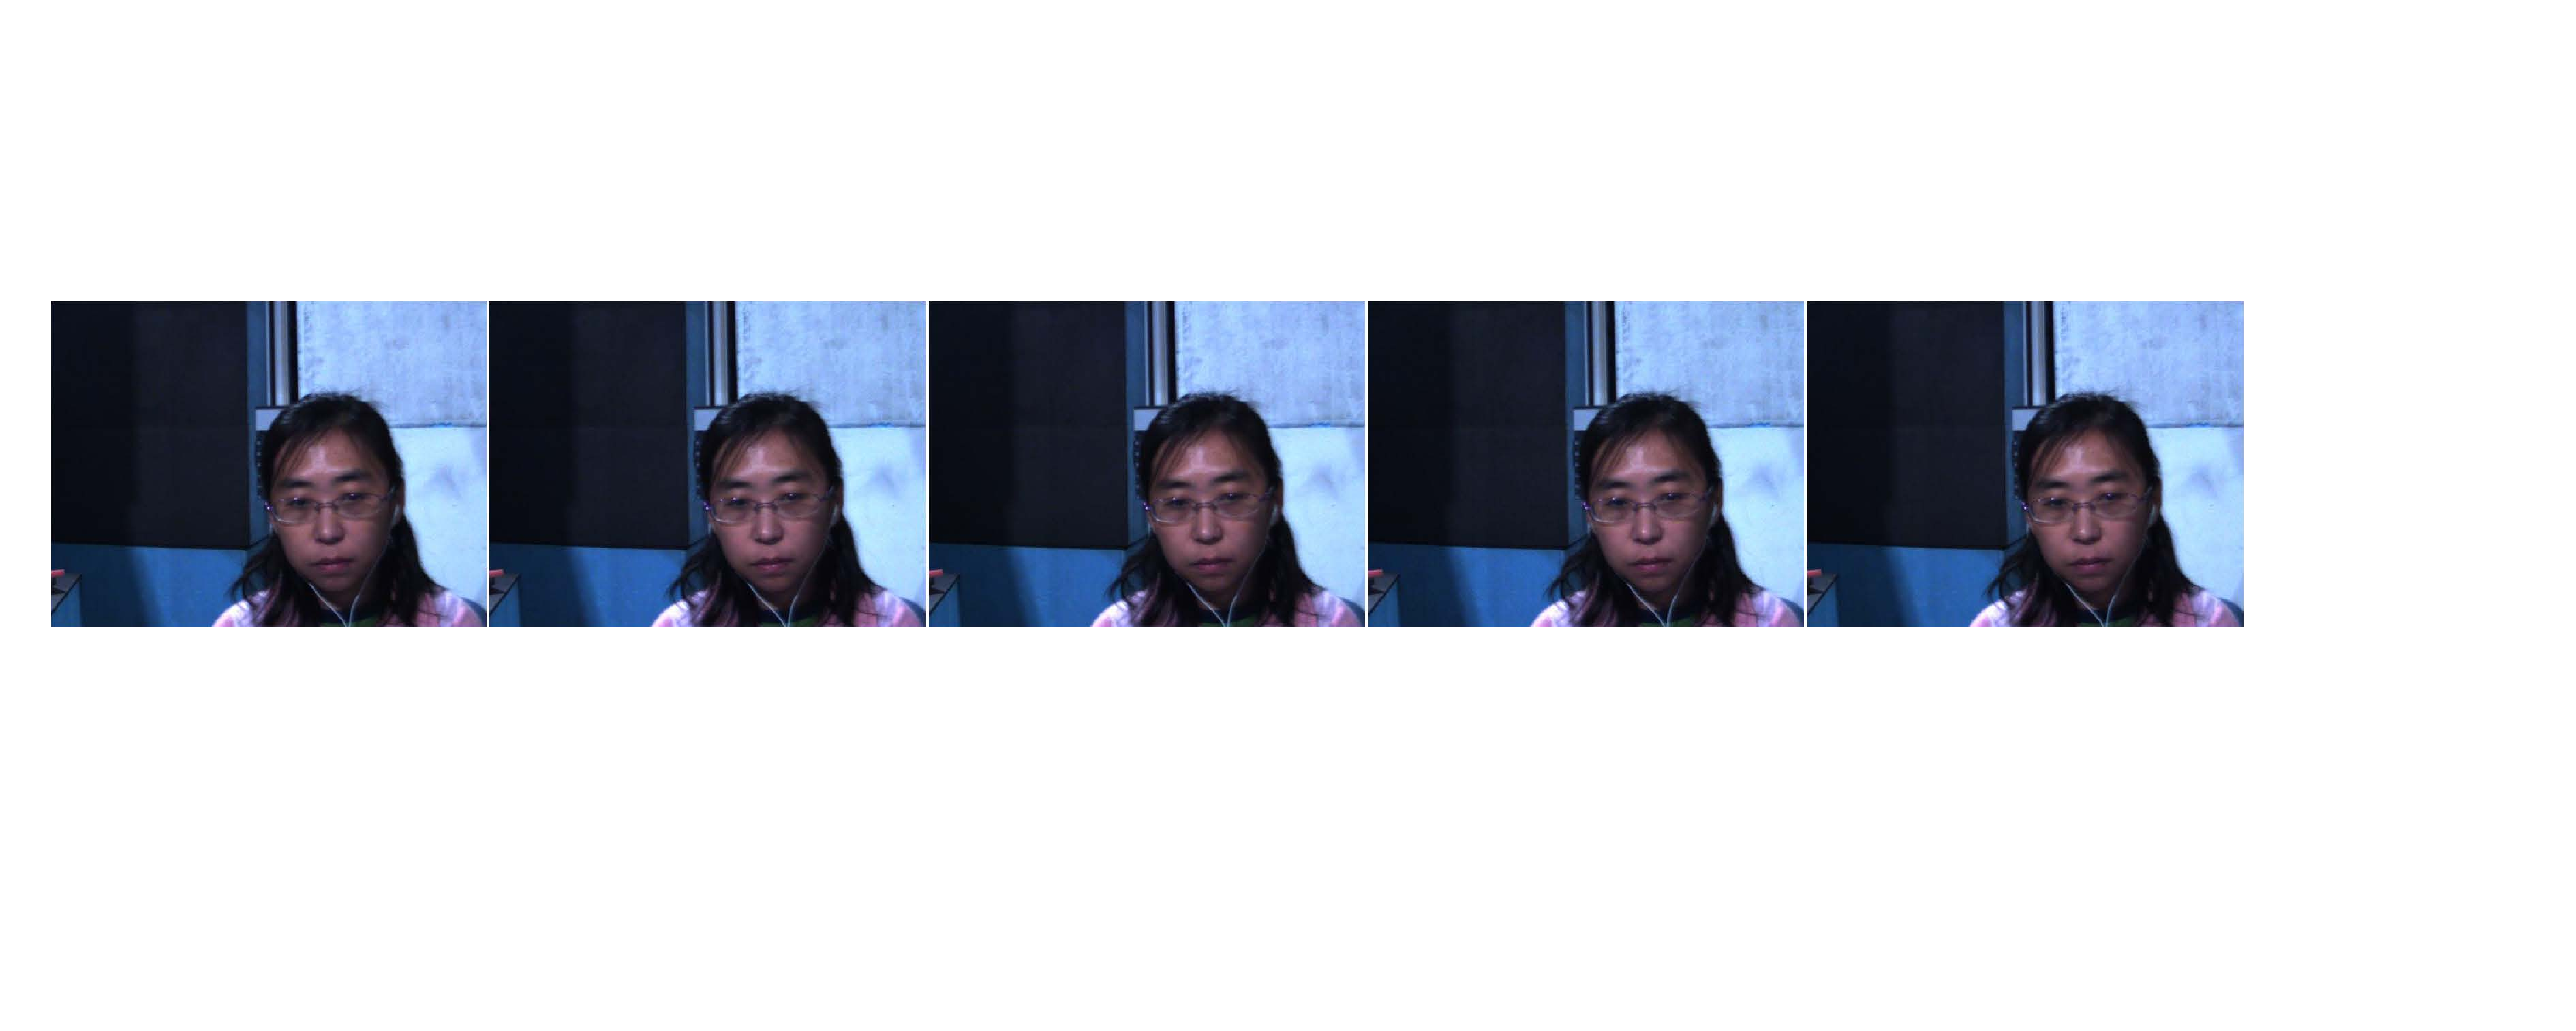
\includegraphics[width=0.95\textwidth]{ME1}
    \caption{一个消极的微表情片段示例(SMIC数据集)}
    \label{fig2}
\end{figure}


a)视频采集

研究表明通过图像、视频和音乐等一定的刺激能够诱发真实的表情\citep{Coan2015Handbook}。自发微表情是由人的内心感受触发的非自愿行为,所以可以使用上述方法引发情感反应。但必须找到一种能确保诱发的表情足够短的方法(满足微表情的标准)。一些心理学著作研究了微表情发生的条件,Ekman等人认为当人们试图隐藏自己的真实情感时,尤其是当被抓住后果会很严重时,微表情就会出现,这被称为高风险条件,例如嫌疑人正在接受警察或测谎专家的审问,这是一种很自然的高风险场景。但是对于采集数据而言,营造真正的审问现场显的不太可能。所以为了诱导参与者自发的微表情,需要找到一种模拟高风险环境的方法。设计的情景必须满足以下两个要求:(1)激发参与者情绪的刺激必须有效,使激发的情绪反应强烈到无法完全隐藏;(2)应该制造高压力,这样参与者才会有动力去尽力隐藏自己的真实感受。

作者使用了心理学研究中诱导抑制情绪产生的方法。采集前向参与者详细说明研究内容和过程,显示器上显示如下提示性语句:“(1)将向您展示几段诱发情绪的短片,请尽量保持头部稳定并仔细观看。(2)每段视频片段后,您将有一个短暂的休息。请根据您对刚才看到的视频的真实感受填写调查表(报告中的情感反馈是标注过程中的重要参考。)。(3)当您在看视频的时候,我会待在另一个房间,通过摄像头观察您的面部和身体动作,并尝试猜测您所看的视频片段(片段是随机播放的)。您的任务是装出若无其事的样子,而不是表露您的真实感情。如果您不能隐藏您的感觉,您将不得不填写一份超过500个冗长而乏味的问题问卷。”

在每段影片结束后,参与者将在问卷中回答以下问题:“(1)您在看视频时感受到了什么样的情绪(快乐、悲伤、厌恶、恐惧、惊讶、愤怒或困惑)?(2)看视频的时候您是否感觉到愉悦?(从1到7愉悦程度逐渐上升)”。选择最有效的刺激作为情感诱导因子是后续数据采集的关键因素之一。通过查阅文献比较不同类型的情绪诱导材料,如图像、音乐、视频和互动。最终决定使用短视频作为微表情采集诱导剂的原因有三个:(1)视频包含音频和视觉信息,因此比图像和音乐的影响更强大;(2)视频能够持续一段时间,更能激发强烈情绪,更容易产生微表情;(3)从获取稳定额叶面部视频的实际角度来看,观看视频的参与者比多人参与的互动场景更容易控制。

20名来自奥卢大学的学生和研究人员自愿参与数据集的制作,参与者的年龄从22岁到34岁不等,其中7位是女性,13位是男性,9人是白种人,11人是亚洲人。研究人员在电脑显示器上向参与者展示了16段精心挑选的能引发强烈情绪的视频片段。当参与者观看视频片段时,三个固定在电脑显示器上的摄像头记录参与者的面部反应,操作人员在前方通过另外一台电脑监控参与者的面部反应,图~\ref{fig3}给出了环境设置示意图。

\begin{figure}[!htbp]
    \centering
    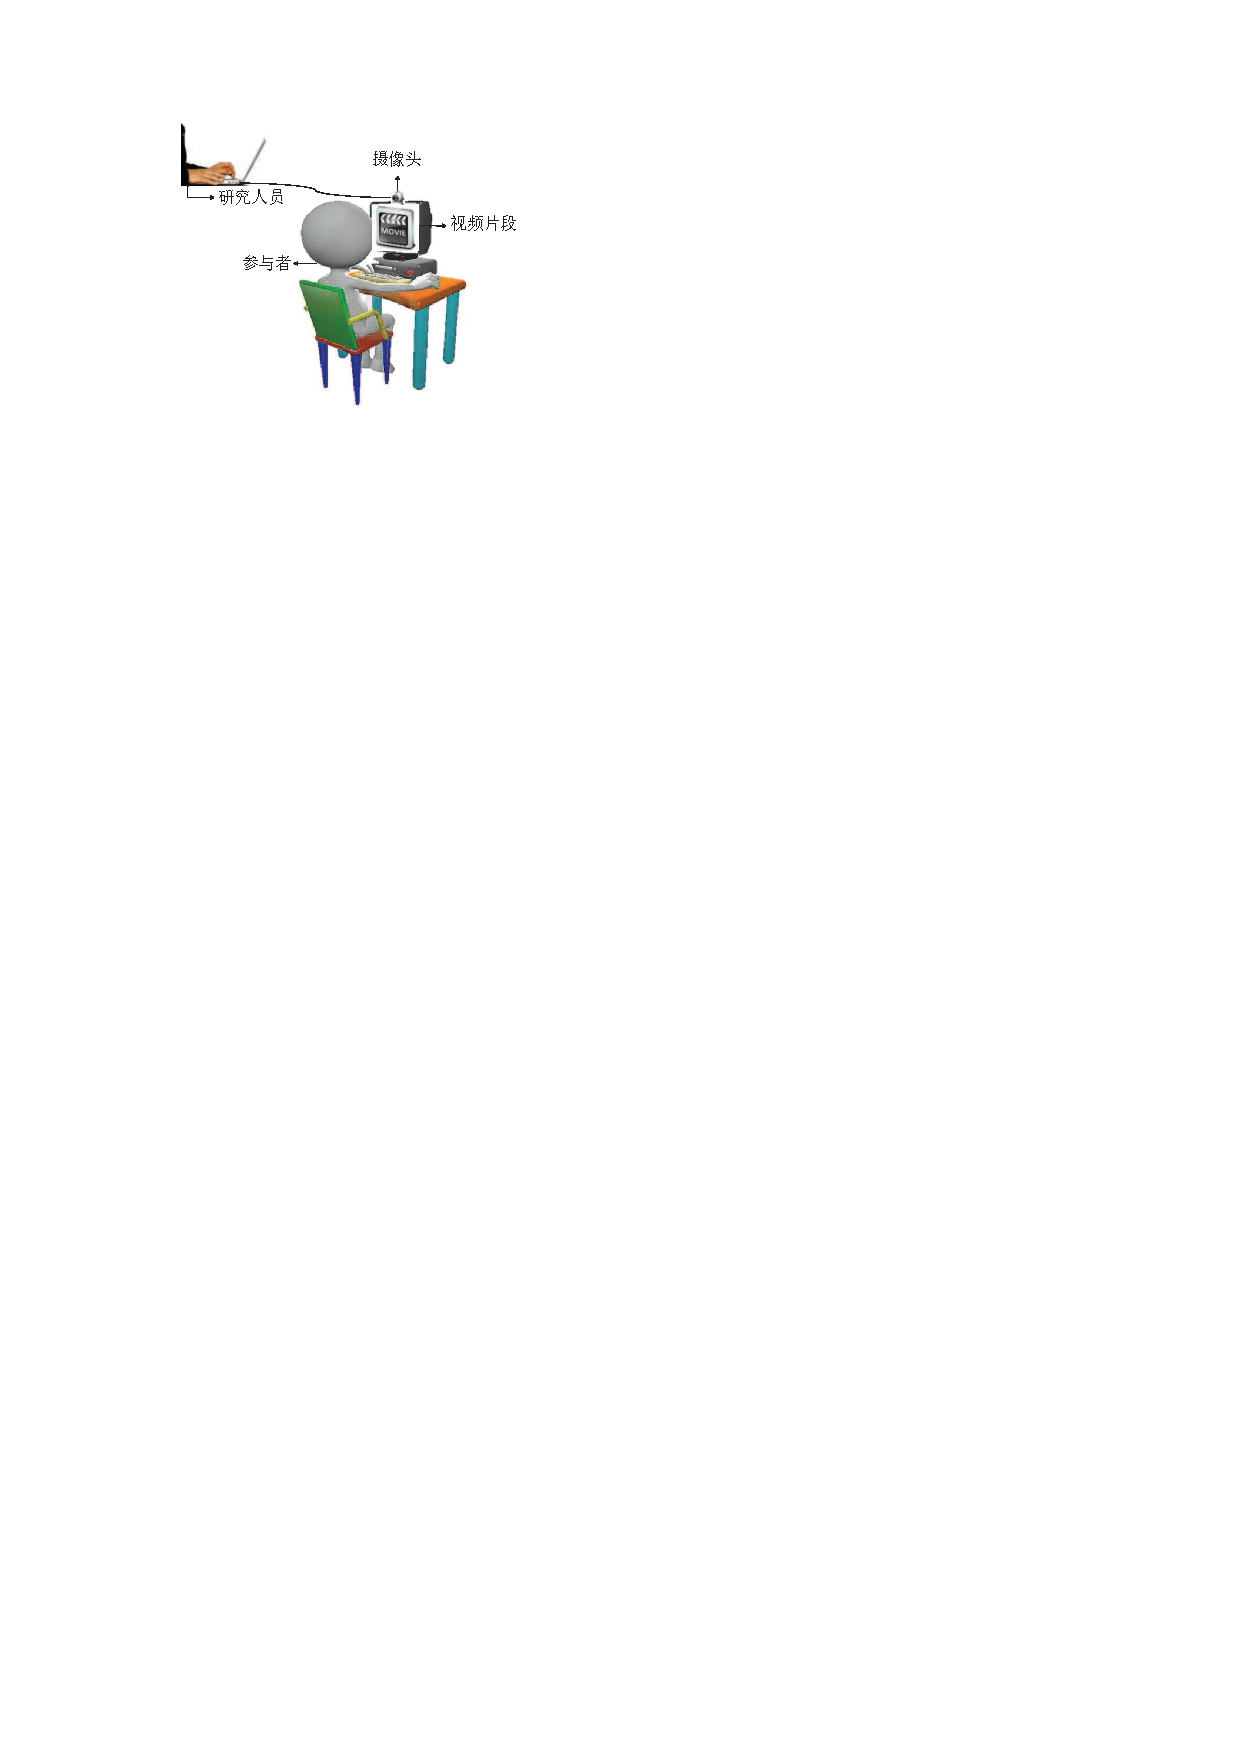
\includegraphics[width=0.45\textwidth]{collect}
    \caption{微表情数据采集示意图}
    \label{fig3}
\end{figure}

b) 视频的标注

录制的视频需要进行分割和标注,目的是得到适合研究人员进行训练与测试的微表情样本和相应的标签。采集的三种视频中高速视频由于具有最佳的时间分辨率所以非常适合标注,另外两个摄像头拍摄的视频需要同步后再进行标注。首先,从原始的长视频中分割出微表情的起始和终止帧,微表情序列的开始表示的是与之前中立(或接近中立)的人脸表情相比的可见运动的第一帧,而微表情序列的终止指在与下一帧相比可以发现任何运动时结束的最后一帧。关于微表情精确的长度限制目前还存在争议,SMIC数据集参考论文\citepns{Yan2013How}和 \citepns{matsumoto2011evidence}等人的建议,设置了1/2秒较宽松的分割节点。注意,并不是所有的微表情都结束于一个完全的中性表情,有些表情可能会上升,然后下降到接近中性的状态,并保持这种状态很长时间,这也被认为是微表情的结束。

随后,对所有的视频片段都用情感标签进行标注。情感标签的证据有两种:视频片段的内容和参与者提交的报告。虽然在视频播放前已经预知将可能产生某种确定情绪,但研究发现,参与者在某些视频刺激下可能会产生不同的情绪表现(甚至相反的情绪)。在少数情况下,当参与者提交的问卷报告与视频内容相反时(例如,一些参与者反馈在观看恐怖视频片段时感到快乐或有趣),SMIC数据集使用参与者的提交的报告作为微表情标签的标准。起初,SMIC数据集根据视频内容分配了五种情感标签,包括快乐,悲伤,恐惧,厌恶,惊讶。后来,SMIC数据集将五类标签合并为三类:积极(Positive)、惊喜(Surprise)和负面(Negative)。将第一版本的快乐类别改为新的积极类别,而消极类别则是由第一版的悲伤、恐惧和厌恶这三个类别组合而成。将三种消极情绪融合在一起的原因是:首先,参与者在该段视频的报告中选择了三种情绪中的一种以上;其次,三种标签的样本量都太小,合并后会更好的平衡。根据具体情况,惊喜类别可以分为正面惊喜和负面惊喜。同时为了验证数据标签的有效性,标注由两位标注者分别执行。然后,两位标注者相互交换检查各自的标注,只有当两位标注者的标注结果一致时的标签有效。

B. CASMEC数据集介绍

在SMIC发表后不久,另一组研究人员收集了新的自发微表情数据集。由中国科学院Yan等人采用与SMIC相似的情绪诱导方式收集的中国科学院微表情数据集(CASME),包含19位中国参与者的195个微表情片段。CASME由两台相机记录,一台是明基M31相机,帧率为60fps,分辨率为$1280\times720$(CASME-A),另一台是灰点GRAS-03K2C相机,帧率为60fps,分辨率为$640\times480$(CASME-B)。CASME数据集中的微表情首先使用AU标记,然后被分为八类情绪,包括娱乐、悲伤、厌恶、惊讶、蔑视、恐惧、压抑和紧张。之后又发布了第二版数据集CASME II,CASME II提供了更多具有更高时空分辨率的微表情样本。新数据集的平均人脸尺寸为$280\times340$,每秒200帧,是从26名中国参与者中获得的247个微表情样本。CASMEII样本有五个类的AU标签和情感标签,即幸福、厌恶、惊讶、压抑和其他。

CASME II数据集相比之前的数据集引入了AU标签,它是在充分考虑了主客观因素(除了FACS编码的基本判断)外,还参考了参与者自己的主观回忆来辅助判断样本标签。除此之外,该数据集还对微表情的起始帧、峰值帧和终止帧都做了详细的标注。

C. 其他数据集介绍

最近又有一个自发微表情的数据集SAMM也使用了类似的情绪诱导方法,从13个不同民族的32名参与者中获得159个微表情。SAMM数据具有更高的帧分辨率$2040\times340$,帧速率为200fps。数据提供了AU标签和七种表情标签,包括生气、开心、蔑视、恐惧、惊讶、厌恶和其他。

表~\ref{tab1}列出了当前所有提到的微表情数据集的详细参数。

\begin{table}[!htbp]
  \centering
  \caption{自发微表情数据集}
  \label{tab1}
  \footnotesize% fontsize
  \setlength{\tabcolsep}{4pt}% column separation
  \renewcommand{\arraystretch}{1.2}%row space
  \begin{tabular}{c|cccccc}
    \hline
     & SMIC-HS & SMIC-subHS & SMIC-NIR & SMIC-VIS & CASME II & SAMM \\ \hline
    微表情片段 & 164 & 71 & 71 & 71 & 247 & 159 \\
    参与者 & 16 & 8 & 8 & 8 & 26 & 32 \\
    分辨率 & $640\times480$ & $640\times480$ & $640\times480$ & $640\times480$ & $640\times480$ & $2040\times1088$ \\
    人脸分辨率 & $190\times230$ & $190\times230$ & $190\times230$ & $190\times230$ & $280\times340$ & $400\times400$ \\
    FPS & 100 & 100 & 100 & 100 & 200 & 200 \\
    性别比(F/M) & 6/10 & 2/6 & 2/6 & 2/6 & 15/11 & 16/16 \\
    FACS & NO & NO & NO & NO & YES & YES \\
    表情类 & 3 & 3 & 3 & 3 & 5 & 7 \\
    平均年龄(SD) & 26.7(N/A) & 26.7(N/A) & 26.7(N/A) & 26.7(N/A) & 22.03(SD=1.6) & 33.24(SD=11.32) \\
    人种 & 2 & 2 & 2 & 2 & 1 & 4 \\ \hline
    \end{tabular}
\end{table}

\subsection{宏表情与微表情比较}

目前存在的宏表情和微表情数据集形式多样,各具特色。但受限于理论研究的不统一,各个数据集的成果迁移性较差,存在着较多的局限性,目前数据集存在的问题主要体现在:

首先,建库标准不一致。对于常用的宏表情数据集,例如JAFFE和CK+两个常用的数据集,他们对情感分类的标准并不一样,JAFFE将表情分为高兴、生气、悲伤、厌恶、惊讶、恐惧、中性7类,而CK+在此基础上加入了蔑视这一类情感。对于微表情数据集,他们的诱发方式不同,有的数据集使用自然诱发,有的使用非自然状态的模拟得到;SMIC数据集并没有对AU单元进行标注,CASME的光照并非自然光照,会与真正的自然光照下的微表情存在一定的差异;另外,不同的数据集根据研究需要,在情感标签分类上也有较大的不同。例如,SMIC微表情数据集将情感分类为积极、消极、惊讶三类,而CASME系列将情感分类高兴、惊讶、悲伤、厌恶、恐惧、抑制和其他七种类型;不同的建库标准导致难以使用统一的方法对数据集进行性能评价。

其次,样本数量有限。目前各个数据集的样本数量较少,尤其是受试者的数量有限,导致数据集的样本数量不够,难以有较强的说服性。微表情数据集目前的样本数量都比较少,不具有普遍意义。

\begin{figure}[!htbp]
    \centering
    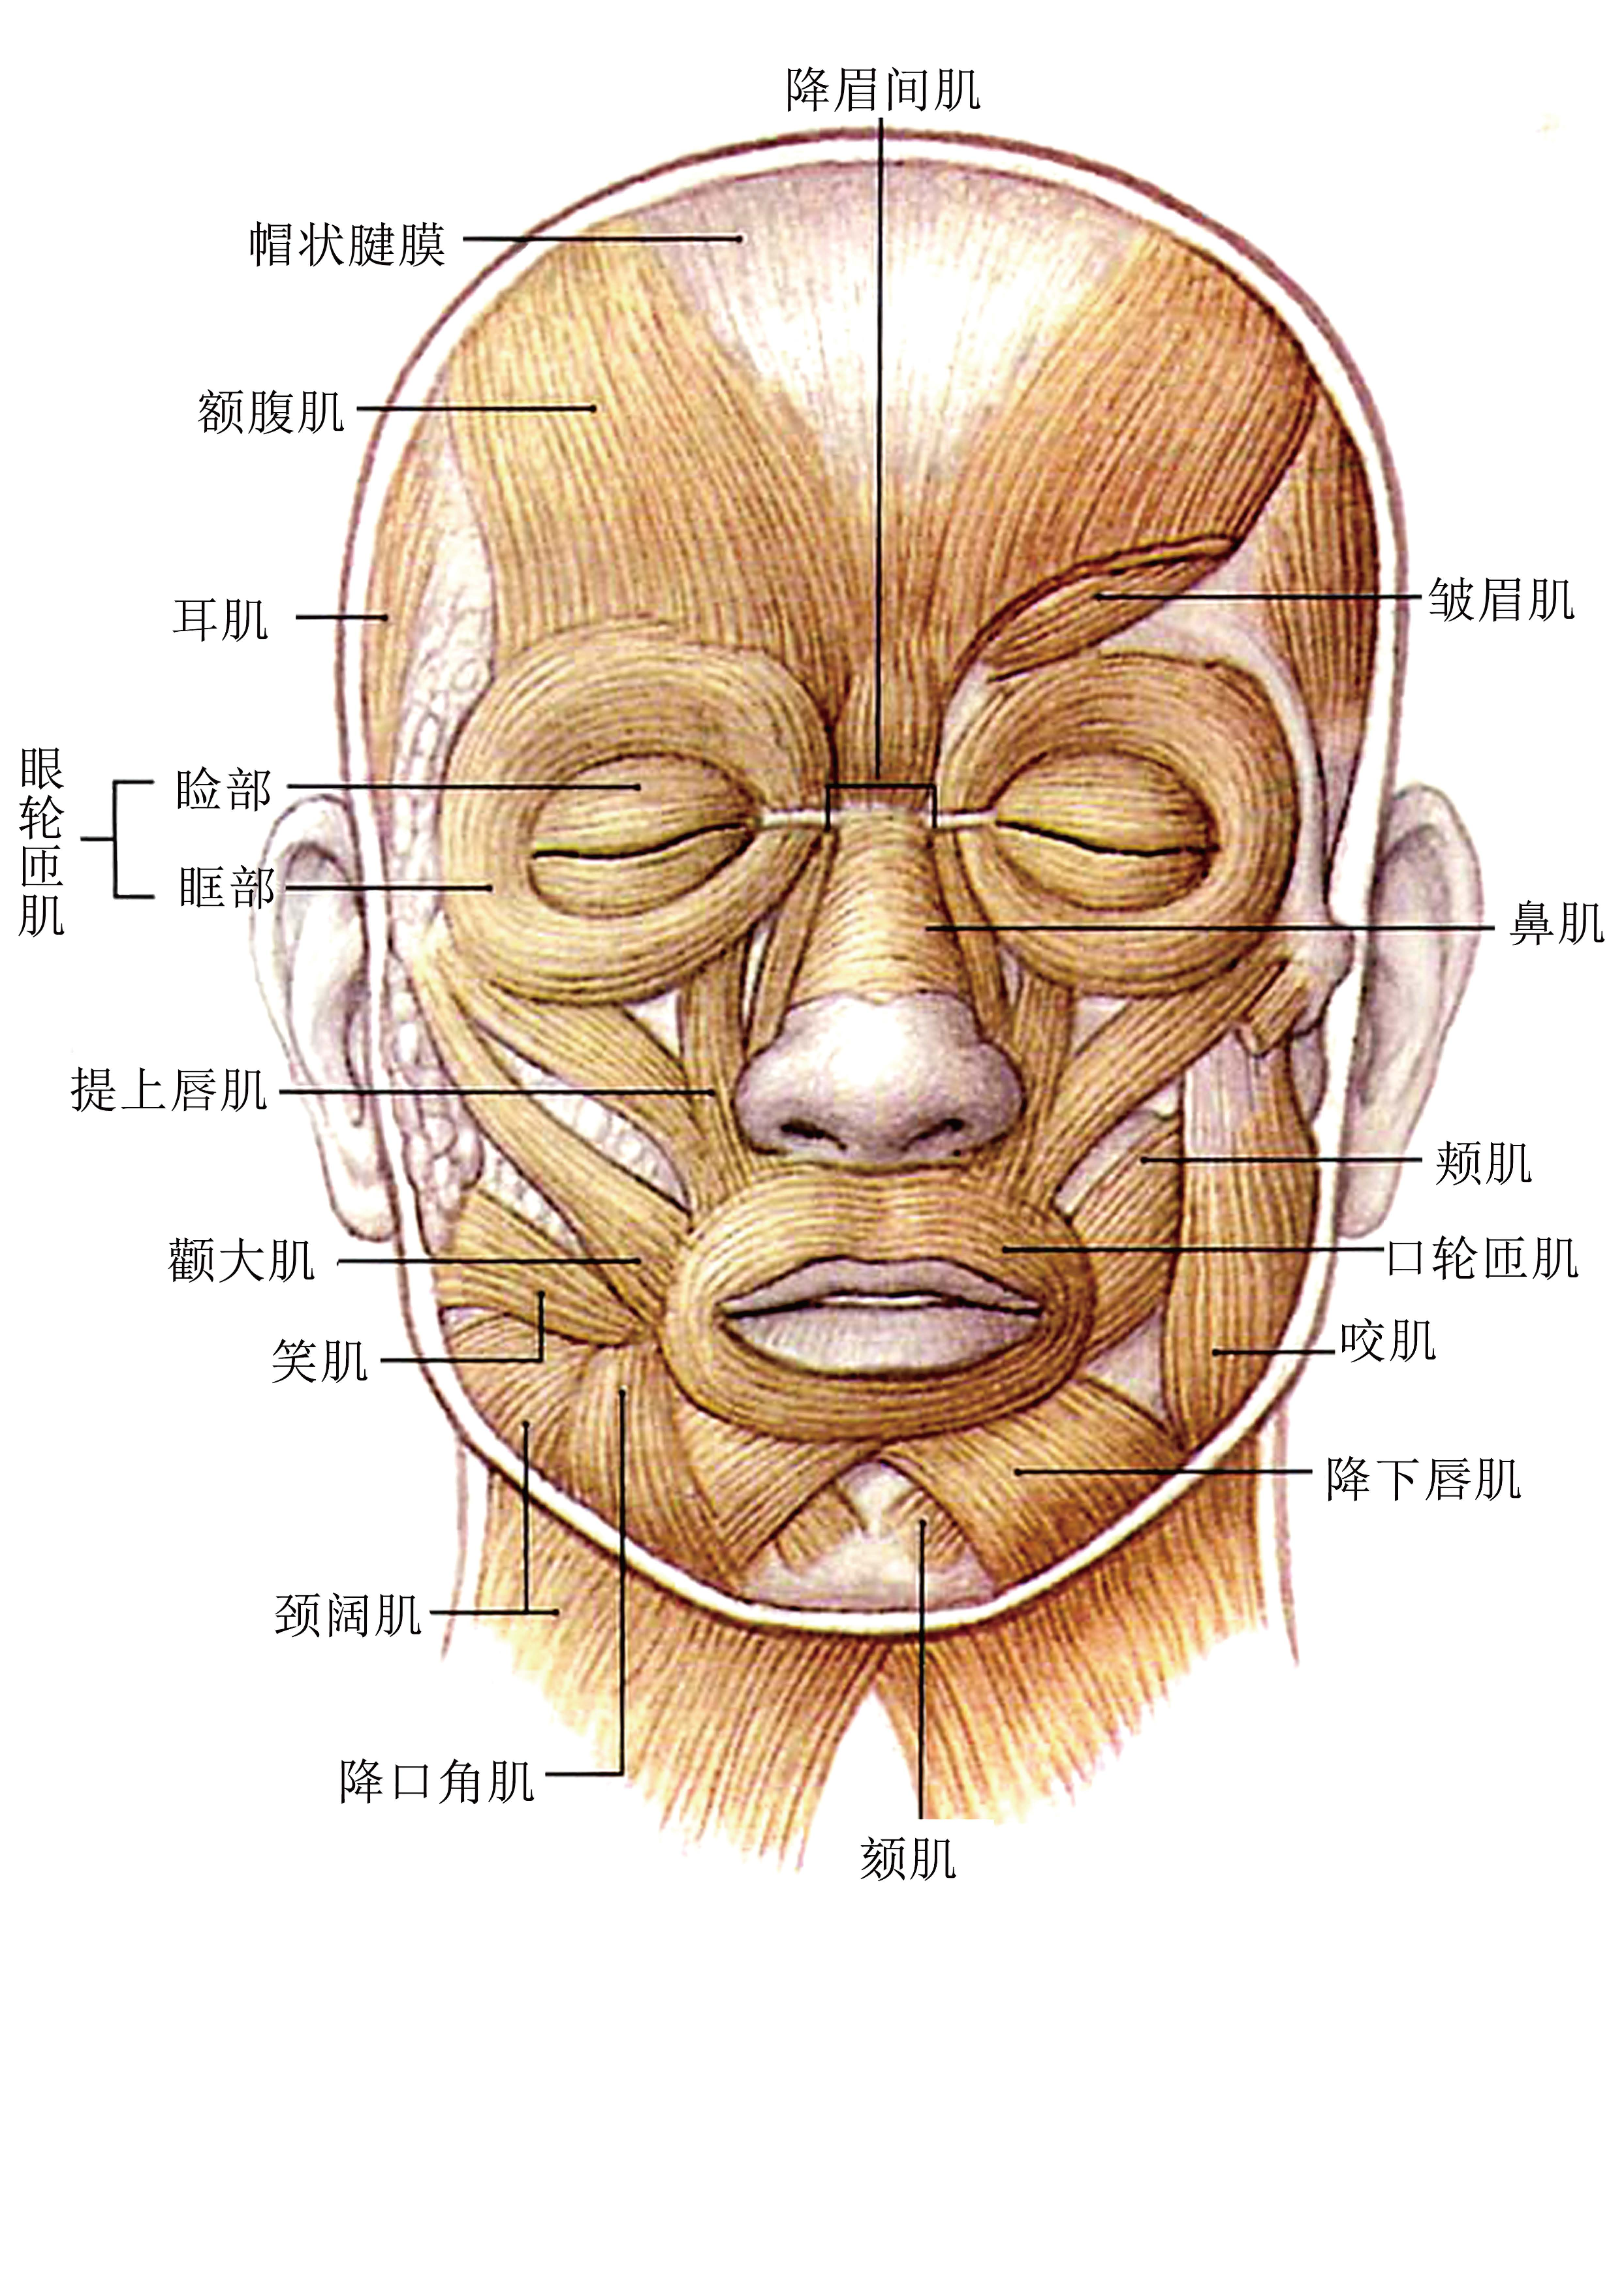
\includegraphics[width=0.25\textwidth]{ME2}
    \caption{人脸面部肌肉划分}
    \label{fig4}
\end{figure}

\section{微表情特征提取的一般方法}

\subsection{LBP-TOP}

LBP可以有效地处理光照变化,在纹理分析,纹理识别方面被广泛应用。

但是LBP 只能处理单张的二维图像,对于视频或者图像序列,如何用LBP来提取特征,捕捉视频序列的运动信息呢。今天我们就介绍一种称为 LBP-TOP 的特征,是芬兰奥卢大学的 Guoying Zhao 等人提出来的,最早是用来处理动态纹理的识别,但是现在已经被广泛用在基于视频的人脸表情识别上面。

LBP-TOP 是 LBP 从二维空间到三维空间的拓展,LBP-TOP 的全称为: local binary patterns from three orthogonal planes, 这里的three orthogonal planes 指的就是三个正交平面,我们知道,单张的图像只有X, Y两个方向,而一个视频或者图像序列除了X,Y 方向之外,还有一个沿着时间轴 T 的方向, 而 X-Y, X-T 和 Y-T 三个方向是相互正交的。

\subsection{光流法}

光流的概念是Gibson在1950年首先提出来的。它是空间运动物体在观察成像平面上的像素运动的瞬时速度,是利用图像序列中像素在时间域上的变化以及相邻帧之间的相关性来找到上一帧跟当前帧之间存在的对应关系,从而计算出相邻帧之间物体的运动信息的一种方法。一般而言,光流是由于场景中前景目标本身的移动、相机的运动,或者两者的共同运动所产生的。其计算方法可以分为三类:

(1)基于区域或者基于特征的匹配方法;

(2)基于频域的方法;

(3)基于梯度的方法;

简单来说,光流是空间运动物体在观测成像平面上的像素运动的“瞬时速度”。光流的研究是利用图像序列中的像素强度数据的时域变化和相关性来确定各自像素位置的“运动”。研究光流场的目的就是为了从图片序列中近似得到不能直接得到的运动场。

光流法的前提假设:

(1)相邻帧之间的亮度恒定;

(2)相邻视频帧的取帧时间连续,或者,相邻帧之间物体的运动比较“微小”;

(3)保持空间一致性;即,同一子图像的像素点具有相同的运动

这里有两个概念需要解释:运动场,其实就是物体在三维真实世界中的运动;光流场,是运动场在二维图像平面上的投影。

\subsection{Gabor特征}

Gabor 特征是一种可以用来描述图像纹理信息的特征,Gabor 滤波器的频率和方向与人类的视觉系统类似,特别适合于纹理表示与判别。Gabor 特征主要依靠 Gabor 核在频率域上对信号进行加窗,从而能描述信号的局部频率信息。

说到 Gabor 核,不能不提到傅里叶变换。正是靠傅里叶变换,我们才能将信号转换到频率域,才能让Gabor核在频率域去加窗。而在原本的空间域中,一个 Gabor 核实际上就是一个高斯核与正弦波调制的结果,可以看做是高斯核应用在了正弦波的频域部分。

\section{相关深度学习网络}

\subsection{3DCNN}

3D CNN 在视频分类,动作识别等领域发挥着巨大的优势,文章:3D Convolutional Neural Networks for Human Action Recognition,该框架应用于动态表情识别。采用2D CNN对视频进行操作的方式,一般都是对视频的每一帧图像分别利用CNN来进行识别,这种方式的识别没有考虑到时间维度的帧间运动信息。使用3D CNN能更好的捕获视频中的时间和空间的特征信息。

需要注意的是:3D卷积核只能从cube中提取一种类型的特征,因为在整个cube中卷积核的权值都是一样的,也就是共享权值,都是同一个卷积核。我们可以采用多种卷积核,以提取多种特征。

输入层(input):连续的大小为$60\times40$的视频帧图像作为输入。

硬线层(hardwired,H1):每帧提取5个通道信息(灰度gray,横坐标梯度(gradient-x),纵坐标梯度(gradient-y),x光流(optflow-x),y光流(optflow-y))。前面三个通道的信息可以直接对每帧分别操作获取,后面的光流(x,y)则需要利用两帧的信息才能提取,因此H1层的特征maps数量:($7+7+7+6+6=33$),特征maps的大小依然是$60\times40$;

卷积层(convolution C2):以硬线层的输出作为该层的输入,对输入5个通道信息分别使用大小为$7\times7\times3$的3D卷积核进行卷积操作($7\times7$表示空间维度,3表示时间维度,也就是每次操作3帧图像),同时,为了增加特征maps的个数,在这一层采用了两种不同的3D卷积核。

降采样层(sub-sampling S3):在该层采用max pooling操作,降采样之后的特征maps数量保持不变。

卷积层(convolution C4):对两组特征maps分别采用$7\times6\times3$的卷积核进行操作,同样为了增加特征maps的数量,文中采用了三种不同的卷积核分别对两组特征map进行卷积操作。这里的特征maps的数量计算有点复杂。

降采样层(sub-sampling S5):对每个特征maps采用3 3的核进行降采样操作,此时每个maps的大小:$7\times4$。在这个阶段,每个通道的特征maps已经很小,通道maps数量分布情况如下:

gray通道maps数量= gradient-x通道maps数量= gradient-y通道maps数量=3

optflow-x通道maps数量=optflow-y通道maps数量=2;

卷积层(convolution C6):此时对每个特征maps采用$7\times4$的2D卷积核进行卷积操作,此时每个特征maps的大小为:$1\times1$,至于数量为128是咋来的,就不咋清楚了,估计是经验值。

对于CNNs,有一个通用的设计规则就是:在后面的层(离输出层近的)特征map的个数应该增加,这样就可以从低级的特征maps组合产生更多类型的特征。

通过多层的卷积和降采样,每连续7帧图像就可以获得128维的特征向量。输出层的单元数与视频动作数是相同的,输出层的每个单元与这128维的特征向量采用全连接。在后面一般采用线性分类器对128维的特征向量进行分类,实现行为识别,3DCNN模型中所有可训练的参数都是随机初始化的,然后通过在线BP算法进行训练。


\subsection{ResNet}
ResNet在2015年被提出,在ImageNet比赛classification任务上获得第一名,因为它“简单与实用”并存,之后很多方法都建立在ResNet50或者ResNet101的基础上完成的,检测,分割,识别等领域都纷纷使用ResNet,Alpha zero也使用了ResNet,所以可见ResNet确实很好用。

随着网络的加深,出现了训练集准确率下降的现象,我们可以确定这不是由于Overfit过拟合造成的(过拟合的情况训练集应该准确率很高);所以作者针对这个问题提出了一种全新的网络,叫深度残差网络,它允许网络尽可能的加深,其中引入了全新的结构如图~\ref{fig5};

\begin{figure}[!htbp]
    \centering
    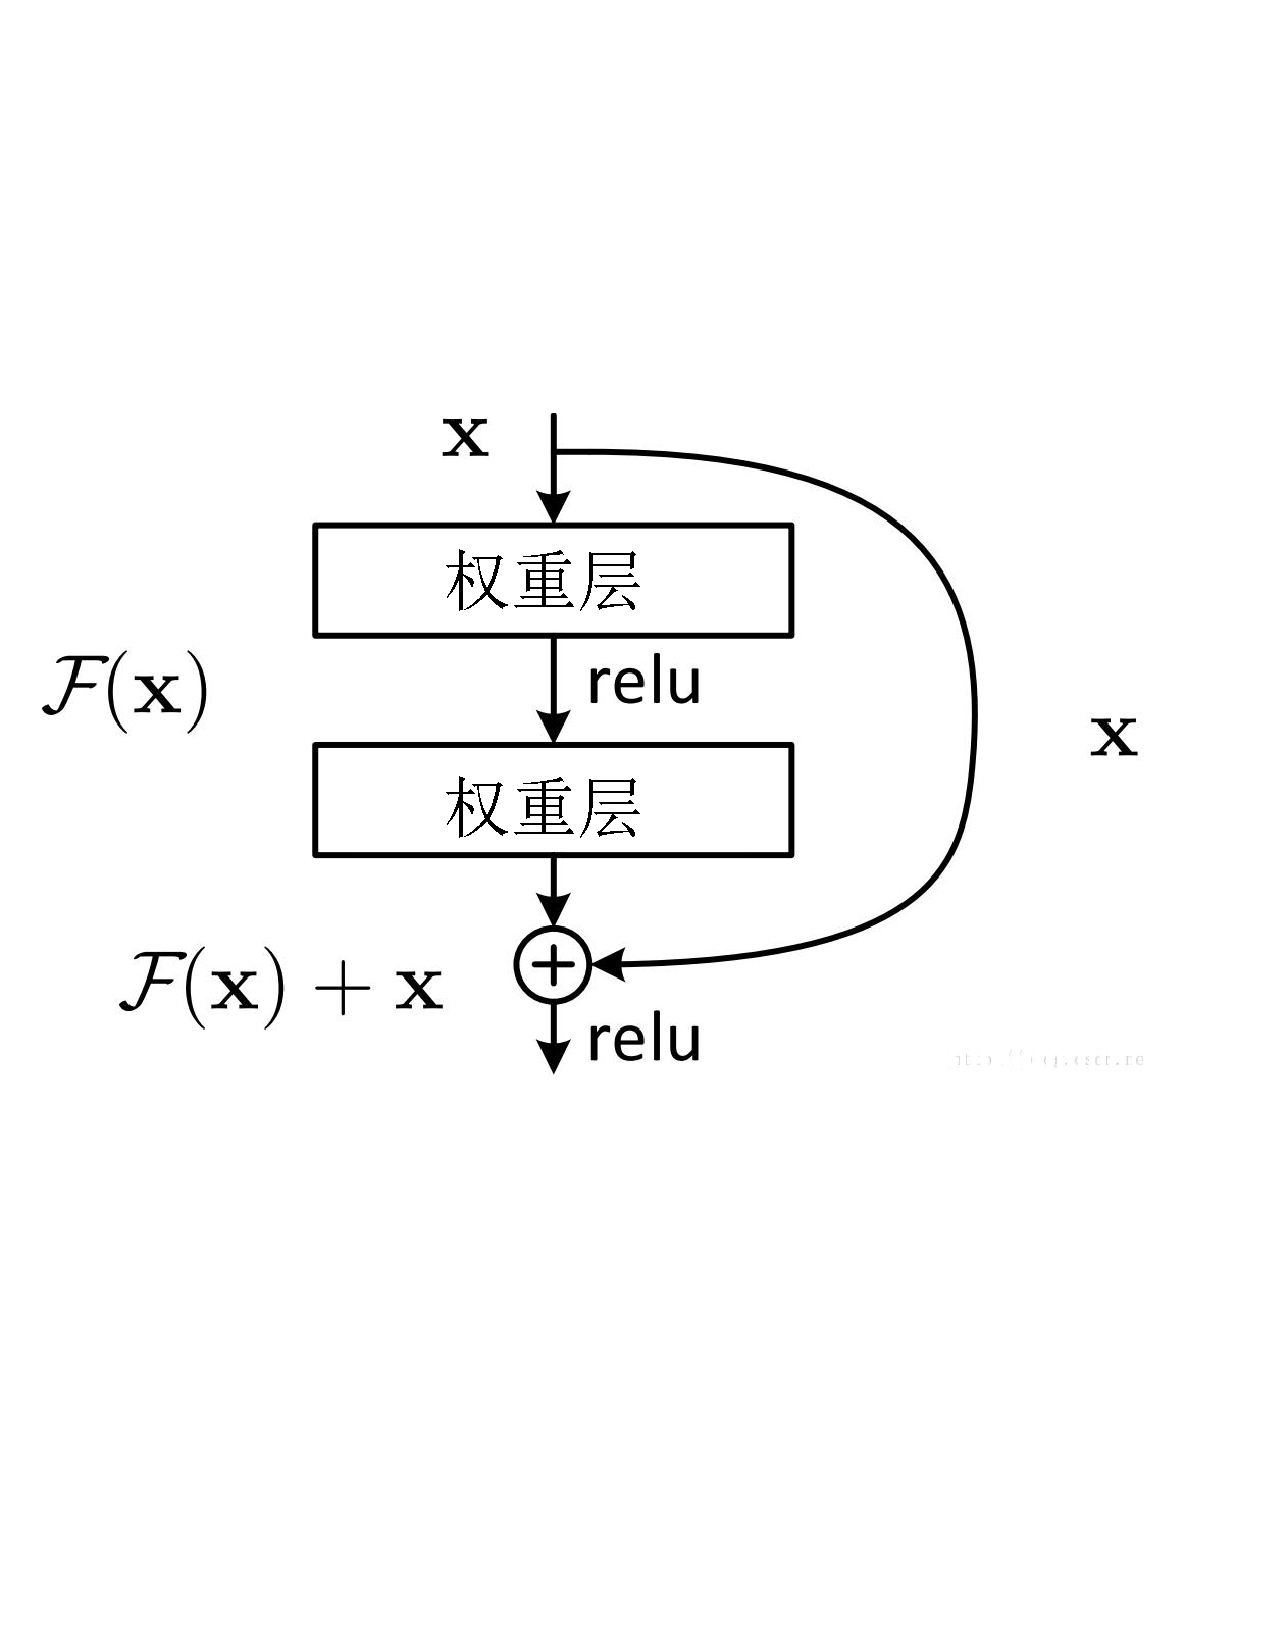
\includegraphics[width=0.50\textwidth]{ME4}
    \caption{ResNet结构图}
    \label{fig5}
\end{figure}
